\documentclass[a4paper,12pt]{article}
\usepackage[utf8]{inputenc}
\usepackage[T1]{fontenc}
\usepackage[brazilian]{babel}
\usepackage{lmodern,microtype}
\usepackage[margin=2.15cm]{geometry}
\usepackage{amsmath,amssymb,booktabs,array,caption,float,graphicx,xcolor}
\usepackage{siunitx,setspace,enumitem,tikz}
\usetikzlibrary{arrows.meta,positioning}
\usepackage[colorlinks=true,linkcolor=blue,urlcolor=blue]{hyperref}
\sisetup{output-decimal-marker={,},group-separator={\,},group-minimum-digits=4}
\setstretch{1.15}
\setlength{\parskip}{3pt}
\setlength{\emergencystretch}{2em}
\captionsetup{font=small,labelfont=bf,skip=4pt}
\setlist{nosep,leftmargin=*}
\newcommand{\cod}[1]{\texttt{\detokenize{#1}}}
\newcommand{\rota}[1]{{\fontsize{8.5}{10.2}\selectfont #1}}
\graphicspath{{figures/}{docs/figures/}}
\title{Trabalho 2 - Material complementar}
\author{João Costa e Miguel Cerne}
\date{Outubro de 2026}
\begin{document}
\maketitle
\begin{abstract}
Material de apoio às análises das Partes 1 e 2. Mantém separados resultados exatos, limites inferiores, projeções de memória e medições de duas rodadas distintas no Azure. O relatório de cinco páginas está em \path{docs/relatorio_parte2.tex}; este complemento não é parte desse limite e não resolve a ausência de tempos de Dijkstra por vetor nos maiores grafos.
\end{abstract}
\setcounter{tocdepth}{1}\tableofcontents
\clearpage
\section{Escopo, arquivos e critérios de cobertura}
O conjunto ponderado é o já medido: Grafos Ponderados 3, 4, 5, 6 e 7, mais a rede de colaboração. Os Grafos Ponderados 1 e 2 de um acervo de 2025/2 não foram incorporados a esta rodada. O enunciado consultado está identificado como COS242, 2025/2; a data deste material e dos experimentos é outubro de 2026. As exigências do documento são tratadas como critérios do relatório, não como autorização para novas execuções de custo elevado.
\par\smallskip\noindent\begin{minipage}{\textwidth}\centering
\begingroup\small
\setlength{\tabcolsep}{4pt}
\begin{tabular}{>{\raggedright\arraybackslash}p{8.3cm}>{\raggedright\arraybackslash}p{7cm}}
\toprule
Exigência da Parte 2 & Situação neste material \\
\midrule
Representação não direcionada com pesos reais & Implementada em CSR e matriz \\
Dijkstra por vetor e por heap atualizável & Ambos implementados e testados \\
Aviso para pesos negativos & Rejeição nas rotinas de Dijkstra \\
Distâncias e caminhos 10 até 20/30/40/50/60 & 25 pares completos no relatório \\
Cinco destinos da rede, com grafia exata & 5 pares completos no relatório \\
Tempos médios das duas versões por grafo & Vetor medido no 3; pendente nos 4 a 7 \\
URL do código e limite de cinco páginas & No relatório principal \\
\bottomrule
\end{tabular}
\endgroup
\end{minipage}\par\smallskip

Não se substituem tempos ausentes por números dos colegas, extrapolações quadráticas ou tempos da versão com entradas obsoletas. A fonte pública do código é \url{https://github.com/Cerne17/graph-library-cpp}. Os dados brutos da nova rodada estão em \path{data/azure_traversals/}; tabelas compactas ficam em \path{docs/results/traversals/}.
\section{Arquitetura e decisões de implementação}

\begin{center}
\begin{tikzpicture}[>=Stealth,box/.style={draw=black!55,rounded corners,align=center,font=\scriptsize,minimum height=8mm,text width=4.4cm},node distance=7mm and 12mm]
\node[box] (pol) {Políticas: direção e ponderação};
\node[box,right=of pol] (io) {Leitura: arestas e mapa de nomes};
\node[box,below=of pol] (storage) {Armazenamentos: CSR e matriz};
\node[box,below=of io] (concept) {Contratos: \texttt{graph\_like}, \texttt{weighted\_graph}};
\node[box,below=of storage] (alg) {Funções livres: buscas e Dijkstra};
\node[box,below=of concept] (heap) {Heap indexado e resultados \texttt{dist}/\texttt{parent}};
\draw[->] (pol)--(storage);
\draw[->] (io)--node[above,sloped,font=\tiny]{constrói}(storage);
\draw[->,dashed] (storage)--node[above,font=\tiny]{satisfaz}(concept);
\draw[->,dashed] (alg)--node[above,sloped,font=\tiny]{requer}(concept);
\draw[->] (alg)--node[above,font=\tiny]{usa / produz}(heap);
\end{tikzpicture}
\captionof{figure}{Arquitetura da biblioteca nova. Setas tracejadas representam contratos verificados em compilação, não herança virtual. O diagrama Mermaid detalhado está em \protect\path{docs/diagrama_classes_atual.mmd}.}
\end{center}

\subsection{Contratos, políticas e armazenamento}
A base legada permanece separada em \path{include/graph.hpp}, \path{src/} e nos aplicativos sem sufixo ponderado. A biblioteca nova ocupa \path{include/graph/}. \cod{graph_like} exige contagem de vértices e visita de vizinhos; \cod{weighted_graph} acrescenta tipo de peso, visita de arestas e detecção de pesos negativos. São restrições estáticas sobre tipos, não classes abstratas. Os aliases de grafo não acrescentam uma camada de objetos sobre os armazenamentos.

Em CSR, o intervalo de vizinhos de $u$ é delimitado por \cod{offsets[u]} e \cod{offsets[u+1]}. As duas orientações de cada aresta são armazenadas nos grafos não direcionados. Destinos e pesos são ordenados juntos. No caso não ponderado, a coluna de pesos é vazia, selecionada em compilação. Arestas paralelas permanecem em CSR; a matriz booleana deduplica adjacências e a matriz ponderada guarda o menor peso de cada par.

A bitmask utiliza $(N+1)\lceil(N+1)/64\rceil$ palavras, cada uma de 8 bytes, com uma linha e coluna zero não usadas. Não se aplica essa mesma economia às células da matriz ponderada: cada célula guarda um número real. Os IDs são de 32 bits, os índices de arestas são de 64 bits e os vértices vão de 1 a $N$.
\subsection{Leitura de entradas compactadas}
Os \emph{harnesses} Python aceitam arquivos \cod{.txt.gz}, validam e descompactam em arquivo temporário, depois fornecem o texto ao programa C++. Isso não é leitura direta de gzip pela biblioteca C++ nem execução de algoritmos sobre conteúdo comprimido. A leitura, a construção e a descompactação ficam fora do intervalo interno de tempo dos algoritmos. O diretório temporário é removido ao terminar. Hashes do texto descompactado permitem verificar que diferentes etapas usaram o mesmo grafo.

O leitor de arestas valida os IDs e campos, aceita comentários e registra os laços descartados. Assim, sua contagem de arestas pode diferir da Parte 1 entregue, que contava laços. A interpretação de pesos negativos refere-se ao grafo após a política de leitura; descartar um laço negativo não equivale a resolver caminhos mínimos no arquivo original. O coletor adicional detecta esse caso; as entradas reais analisadas não contêm pesos negativos.
\subsection{Heap indexado, vetor e entradas obsoletas}
O heap mantém \cod{heap_}, \cod{key_} e \cod{pos_}. Cada troca atualiza as posições dos dois vértices. Inserção, remoção e atualização de chave custam $O(\log N)$; consulta de presença custa $O(1)$. O indexado mantém no máximo uma entrada ativa por vértice. Os vetores de chave e posição são dimensionados para todos os vértices, mesmo se a componente alcançada for pequena.

A versão por vetor varre as estimativas dos não finalizados a cada seleção e para quando não resta distância finita. Com componente alcançada de $N_c$ vértices e $M_c$ arestas, o custo é $O(N+NN_c+M_c)$ em CSR. A implementação com \cod{std::priority_queue} insere uma nova entrada a cada melhoria e descarta uma entrada quando sua distância ficou obsoleta; pode usar espaço proporcional às relaxações bem-sucedidas. O heap próprio oferece atualização de chave e cumpre a exigência específica do enunciado; a terceira versão não deve ser confundida com ele.
\subsection{Caminhos, empates e pesos zero}
A distância inicial é infinita, exceto na origem; o vetor de pais começa em zero. Uma melhoria estrita atualiza distância e pai. Isso evita substituir pais apenas por empate e trata ciclos de peso zero. Inalcançável tem distância infinita e caminho vazio; origem igual ao destino tem caminho unitário. O mapa de nomes usa as grafias exatas e, quando há repetição de nome, resolve para o primeiro ID; esse critério deve ser lembrado ao interpretar nomes ambíguos.
\clearpage
\section{Estrutura e memória dos grafos ponderados}
\par\smallskip\noindent\begin{minipage}{\textwidth}\centering
\begingroup\fontsize{8.4}{10.5}\selectfont
\setlength{\tabcolsep}{4pt}
\begin{tabular}{lrrrrrr}
\toprule
Grafo & $N$ & $M$ & $\delta$ (\%) & Comp. & CSR (MiB) & Matriz (GiB) \\
\midrule
Grafo Ponderado 3 & \num{100000} & \num{6099941} & \num{0.122} & \num{1} & \num{140.55} & \num{74.5} \\
Grafo Ponderado 4 & \num{1000000} & \num{30999978} & \num{0.0062} & \num{1} & \num{717.39} & \num{7.45e+03} \\
Grafo Ponderado 5 & \num{10000000} & \num{39999995} & \num{8e-05} & \num{1} & \num{992.05} & \num{7.45e+05} \\
Grafo Ponderado 6 & \num{10000000} & \num{73403372} & \num{0.000147} & \num{4} & \num{1756.5} & \num{7.45e+05} \\
Grafo Ponderado 7 & \num{50000000} & \num{59999999} & \num{4.8e-06} & \num{1} & \num{1755} & \num{1.86e+07} \\
Rede de colaboração & \num{722385} & \num{2272543} & \num{0.000871} & \num{77486} & \num{57.73} & \num{3.89e+03} \\
\bottomrule
\end{tabular}
\endgroup
\end{minipage}\par\smallskip

A densidade considera os pares distintos; a contagem $M$ preserva as paralelas válidas. O RSS de CSR desta tabela pertence à rodada histórica de Dijkstra; a estimativa matricial representa apenas as células. A diferença entre valor estimado e medido não deve ser atribuída apenas a estruturas matemáticas: o RSS inclui efeitos do alocador, páginas residentes e a medição de uma linha de base.
\par\smallskip\noindent\begin{minipage}{\textwidth}\centering
\begingroup\fontsize{9}{11}\selectfont
\setlength{\tabcolsep}{4pt}
\begin{tabular}{lrrrr}
\toprule
Grafo & Componentes & Maior & Menor & Isolados \\
\midrule
Grafo Ponderado 3 & \num{1} & \num{100000} & \num{100000} & \num{0} \\
Grafo Ponderado 4 & \num{1} & \num{1000000} & \num{1000000} & \num{0} \\
Grafo Ponderado 5 & \num{1} & \num{10000000} & \num{10000000} & \num{0} \\
Grafo Ponderado 6 & \num{4} & \num{9999997} & \num{1} & \num{3} \\
Grafo Ponderado 7 & \num{1} & \num{50000000} & \num{50000000} & \num{0} \\
Rede de colaboração & \num{77486} & \num{576309} & \num{1} & \num{43576} \\
\bottomrule
\end{tabular}
\endgroup
\captionof{table}{Estrutura exata das componentes; conectividade desconsidera os pesos.}
\end{minipage}\par\smallskip
\par\smallskip\noindent\begin{minipage}{\textwidth}\centering
\begingroup\fontsize{9}{11}\selectfont
\setlength{\tabcolsep}{4pt}
\begin{tabular}{lrrrr}
\toprule
Grafo & Grau mínimo & Mediana & Média & Máximo \\
\midrule
Grafo Ponderado 3 & \num{78} & \num{122} & \num{121.999} & \num{171} \\
Grafo Ponderado 4 & \num{25} & \num{62} & \num{62} & \num{102} \\
Grafo Ponderado 5 & \num{2} & \num{8} & \num{8} & \num{25} \\
Grafo Ponderado 6 & \num{0} & \num{15} & \num{14.6807} & \num{38} \\
Grafo Ponderado 7 & \num{1} & \num{2} & \num{2.4} & \num{9} \\
Rede de colaboração & \num{0} & \num{3} & \num{6.29178} & \num{643} \\
\bottomrule
\end{tabular}
\endgroup
\captionof{table}{Graus em CSR, incluindo a multiplicidade das arestas paralelas.}
\end{minipage}\par\smallskip
\par\smallskip\noindent\begin{minipage}{\textwidth}\centering
\begingroup\fontsize{8.8}{11}\selectfont
\setlength{\tabcolsep}{4pt}
\begin{tabular}{lrrrrr}
\toprule
Grafo & Peso mínimo & Média & Máximo & Pesos zero & Paralelas \\
\midrule
Grafo Ponderado 3 & \num{0} & \num{4.95718} & \num{10} & \num{3074} & \num{73} \\
Grafo Ponderado 4 & \num{0} & \num{4.91877} & \num{10} & \num{15950} & \num{34} \\
Grafo Ponderado 5 & \num{0} & \num{4.3746} & \num{10} & \num{24894} & \num{4} \\
Grafo Ponderado 6 & \num{0} & \num{4.99997} & \num{10} & \num{36410} & \num{0} \\
Grafo Ponderado 7 & \num{0} & \num{2.91654} & \num{10} & \num{55177} & \num{0} \\
Rede de colaboração & \num{0.00373459} & \num{5.17518} & \num{113} & \num{0} & \num{0} \\
\bottomrule
\end{tabular}
\endgroup
\captionof{table}{Propriedades das arestas ponderadas válidas.}
\end{minipage}\par\smallskip

O Grafo Ponderado 6 possui três isolados; ``quase conexo'' não significa que todas as origens alcancem todos os vértices. Na rede de colaboração, as muitas componentes pequenas e os isolados contribuem para médias menores que as medianas quando parte das origens sorteadas não alcança a componente gigante. Não há uma regra geral segundo a qual assimetria sempre ``distorce negativamente'' a média: média e mediana resumem aspectos diferentes da distribuição.
\clearpage
\section{Dijkstra: resultados medidos e limites}
\par\smallskip\noindent\begin{minipage}{\textwidth}\centering
\begingroup\fontsize{8.6}{11}\selectfont
\setlength{\tabcolsep}{4pt}
\begin{tabular}{lrrr}
\toprule
Grafo & Vetor & Heap indexado & Entradas obsoletas \\
\midrule
Grafo Ponderado 3 & \num{26.5001} / \num{26.5003} & \num{0.118048} / \num{0.117863} & \num{0.153913} / \num{0.153597} \\
Grafo Ponderado 4 & \textit{Não medido} & \num{2.14328} / \num{2.13201} & \num{2.04099} / \num{2.03725} \\
Grafo Ponderado 5 & \textit{Não medido} & \num{23.6919} / \num{23.7072} & \num{12.827} / \num{12.8327} \\
Grafo Ponderado 6 & \textit{Não medido} & \num{27.7484} / \num{27.7863} & \num{17.9488} / \num{17.9854} \\
Grafo Ponderado 7 & \textit{Não medido} & \num{110.913} / \num{111.1} & \num{40.9326} / \num{40.9552} \\
Rede de colaboração & \textit{Não medido} & \num{0.374306} / \num{0.474432} & \num{0.240864} / \num{0.30788} \\
\bottomrule
\end{tabular}
\endgroup
\captionof{table}{Média / mediana, em segundos, com 100 origens por algoritmo medido.}
\end{minipage}\par\smallskip

A rodada histórica usa o commit registrado em \path{data/azure/environment.txt} (\cod{b414456}), e as distâncias das versões são comparadas fora do intervalo de tempo. Ela conserva médias e medianas agregadas, mas não preserva uma planilha completa de cada origem e tempo individual como a nova coleta. Não é possível reconstruir dela um desvio-padrão confiável; tal campo não foi inventado.

A versão por vetor no Grafo Ponderado 3 fornece uma comparação concreta entre seleção linear e heap. Nos demais grafos, a versão existe e passa nos testes, mas não foi medida. O crescimento quadrático explica a decisão prática de não executá-la; não transforma uma extrapolação em uma medição, nem satisfaz integralmente a tabela exigida pelo enunciado. Seria necessária uma rodada específica para completar essa lacuna.

O fato de a versão com entradas obsoletas superar a indexada nos maiores casos merece investigação por contadores de operações e memória. A implementação indexada acessa posições e chaves por vértice, enquanto a outra armazena pares na fila; localidade e volume de atualizações são hipóteses plausíveis. As tabelas demonstram o resultado observado, não o mecanismo causal.
\begin{figure}[H]\centering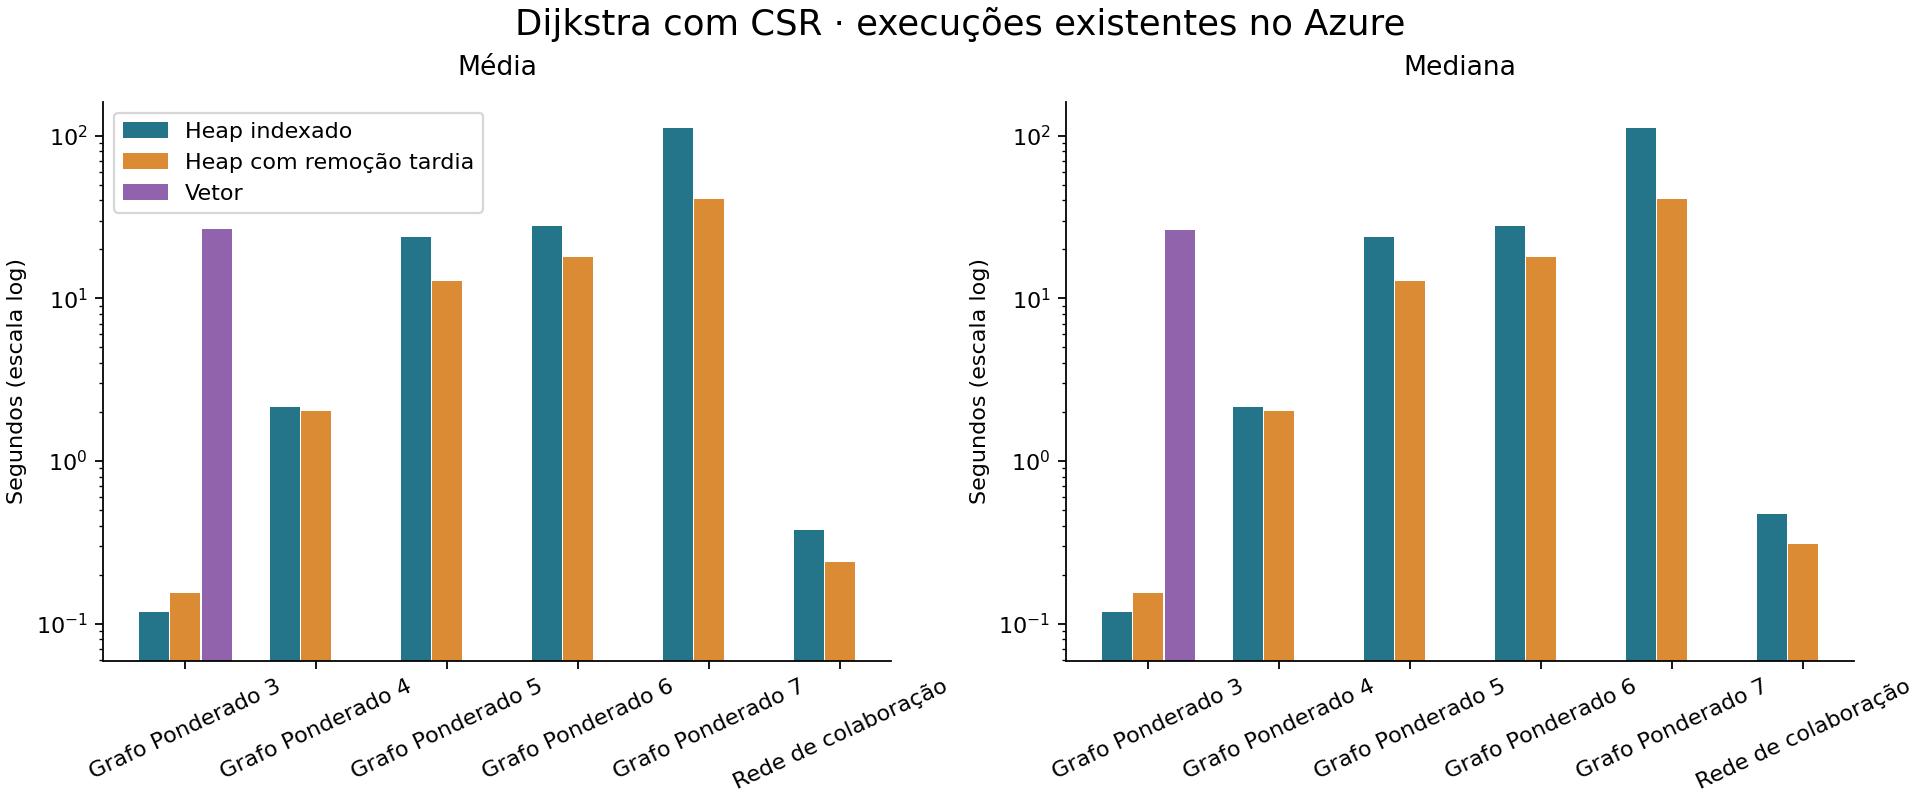
\includegraphics[width=\textwidth]{parte2/azure_timings.png}\caption{Dijkstra no Azure: médias e medianas. Dados ausentes da versão por vetor não equivalem a tempo zero.}\end{figure}
\begin{figure}[H]\centering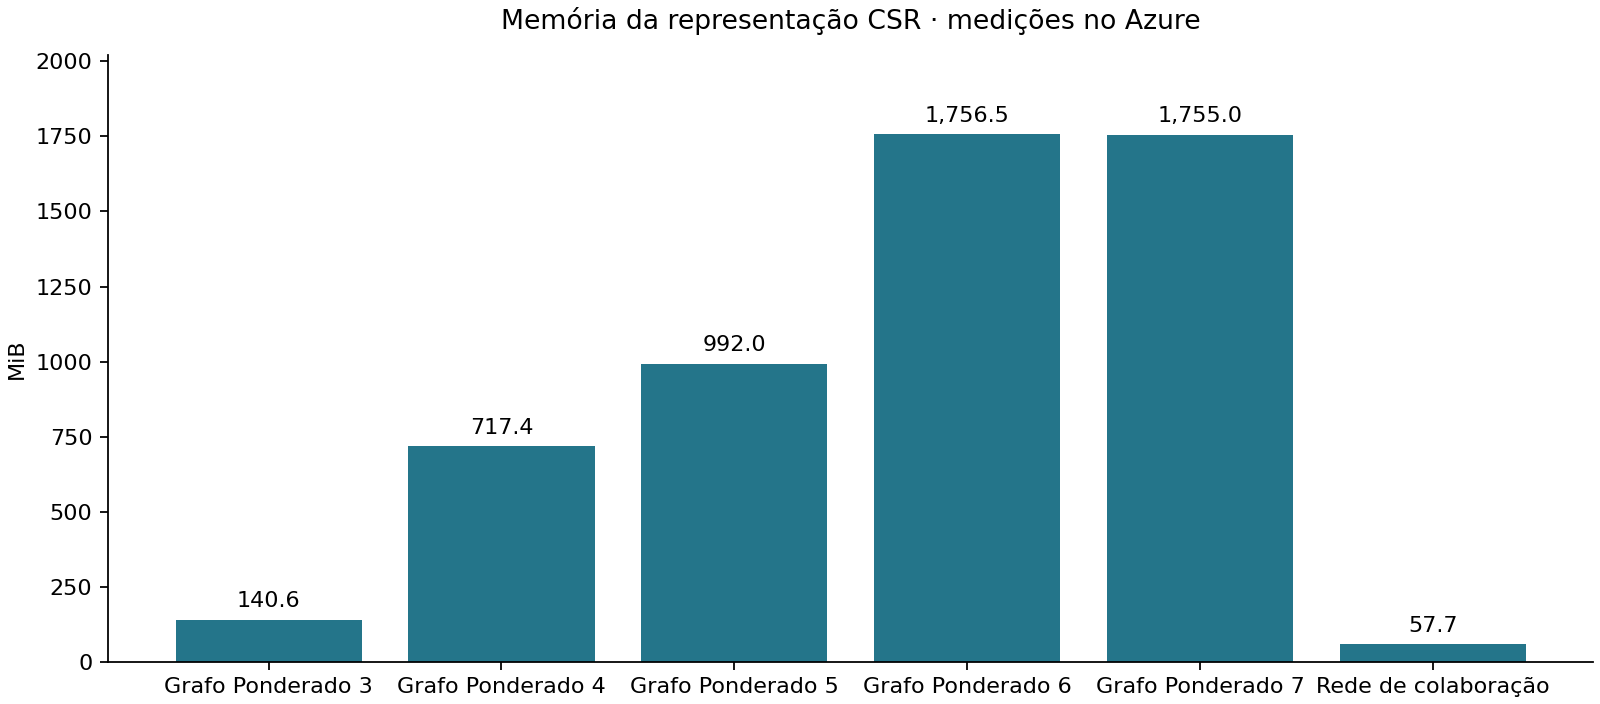
\includegraphics[width=\textwidth]{parte2/azure_memory.png}\caption{Memória residente de CSR na rodada histórica. Não é pico de memória das buscas.}\end{figure}
\clearpage
\section{Busca e comparação com a Parte 1}
\subsection{Protocolo da nova rodada}
A nova rodada de 31/10/2026 foi executada sequencialmente em uma VM da mesma categoria, em \cod{belgiumcentral}, com 4 vCPUs e 32 GiB. Os fontes incluíam alterações locais, preservadas em um snapshot de 99 arquivos com hashes: o commit isolado não representa todo o código medido. São 32 execuções e 2.150 travessias, com semente 2025 e origens distintas. A duração total foi 17 min 27 s; a soma dos intervalos internos das buscas foi 11 min 44 s. Nenhum benchmark de Dijkstra foi repetido nessa rodada.

A quantidade de origens considera número de vértices, arestas, tamanhos das componentes e armazenamento. Para CSR, o trabalho esperado pesa componentes pela probabilidade de uma origem uniforme pertencer a cada uma: $E[N_c]=\sum_i n_i^2/N$. Para a bitmask, considera-se também a varredura de palavras por linha. O ajuste do plano foi feito antes da VM; não selecionou resultados rápidos depois de medi-los. Dez origens fornecem evidência exploratória menos precisa que cem.

BFS e DFS usam a mesma sequência por grafo. Quando CSR possui mais amostras, sua comparação com matriz restringe-se ao prefixo comum. A média CSR completa é publicada separadamente. As 2.150 contagens de alcançados foram conferidas contra os tamanhos exatos das componentes. Hashes verificaram identidade dos dados, do executável e dos artefatos. A VM, disco, IP, rede e permissão temporária foram removidos após o download validado.
\subsection{Tempos completos em CSR}
\par\smallskip\noindent\begin{minipage}{\textwidth}\centering
\begingroup\fontsize{8.7}{10.7}\selectfont
\setlength{\tabcolsep}{4pt}
\begin{tabular}{lrrrrr}
\toprule
Grafo & $k$ & BFS média & BFS mediana & DFS média & DFS mediana \\
\midrule
Grafo 1 & 100 & \num{0.000564842} & \num{0.000563502} & \num{0.00123093} & \num{0.0012252} \\
Grafo 2 & 100 & \num{0.00216596} & \num{0.00320426} & \num{0.00595434} & \num{0.00881832} \\
Grafo 3 & 100 & \num{0.0110273} & \num{0.0126598} & \num{0.0166351} & \num{0.0194219} \\
Grafo 4 & 100 & \num{0.042675} & \num{0.0553162} & \num{0.0670567} & \num{0.0809002} \\
Grafo 5 & 100 & \num{0.336292} & \num{0.498899} & \num{0.531374} & \num{0.771762} \\
Grafo 6 & 50 & \num{0.649268} & \num{0.884291} & \num{0.786941} & \num{1.00465} \\
Grafo Ponderado 3 & 100 & \num{0.0333145} & \num{0.0330618} & \num{0.0570566} & \num{0.0568101} \\
Grafo Ponderado 4 & 75 & \num{0.320946} & \num{0.321259} & \num{0.404246} & \num{0.402048} \\
Grafo Ponderado 5 & 10 & \num{2.2057} & \num{2.20276} & \num{3.41223} & \num{3.39587} \\
Grafo Ponderado 6 & 10 & \num{3.01535} & \num{3.01132} & \num{3.86665} & \num{3.84697} \\
Grafo Ponderado 7 & 10 & \num{10.6629} & \num{10.6406} & \num{16.3364} & \num{16.1243} \\
Rede de colaboração & 100 & \num{0.0447517} & \num{0.0543639} & \num{0.0734379} & \num{0.090937} \\
\bottomrule
\end{tabular}
\endgroup
\captionof{table}{Tempos em segundos; pesos são ignorados por BFS e DFS.}
\end{minipage}\par\smallskip
\clearpage\subsection{Dispersão e alcançabilidade em CSR}
\par\smallskip\noindent\begin{minipage}{\textwidth}\centering
\begingroup\fontsize{8.3}{10.5}\selectfont
\setlength{\tabcolsep}{4pt}
\begin{tabular}{lrrrrrr}
\toprule
Grafo & Busca & Mínimo (s) & Máximo (s) & Desvio (s) & Alc. mín. & Alc. máx. \\
\midrule
Grafo 1 & BFS & \num{0.000546001} & \num{0.000645002} & \num{1.49433e-05} & \num{10000} & \num{10000} \\
Grafo 1 & DFS & \num{0.0012107} & \num{0.0016707} & \num{4.60845e-05} & \num{10000} & \num{10000} \\
Grafo 2 & BFS & \num{4.3e-05} & \num{0.00427631} & \num{0.00133656} & \num{781} & \num{25000} \\
Grafo 2 & DFS & \num{7.42e-05} & \num{0.0136973} & \num{0.00391} & \num{781} & \num{25000} \\
Grafo 3 & BFS & \num{0.00611091} & \num{0.0170855} & \num{0.00328001} & \num{125000} & \num{250000} \\
Grafo 3 & DFS & \num{0.00835442} & \num{0.0253494} & \num{0.00550784} & \num{125000} & \num{250000} \\
Grafo 4 & BFS & \num{0.0215172} & \num{0.0648888} & \num{0.0165101} & \num{125000} & \num{250000} \\
Grafo 4 & DFS & \num{0.0335723} & \num{0.101156} & \num{0.0279863} & \num{125000} & \num{250000} \\
Grafo 5 & BFS & \num{0.0312866} & \num{0.519875} & \num{0.184283} & \num{156250} & \num{2500000} \\
Grafo 5 & DFS & \num{0.044985} & \num{0.819995} & \num{0.289244} & \num{156250} & \num{2500000} \\
Grafo 6 & BFS & \num{0.0310978} & \num{0.893653} & \num{0.316458} & \num{156250} & \num{2500000} \\
Grafo 6 & DFS & \num{0.0666828} & \num{1.15286} & \num{0.358014} & \num{156250} & \num{2500000} \\
Grafo Ponderado 3 & BFS & \num{0.0290323} & \num{0.0397209} & \num{0.00189982} & \num{100000} & \num{100000} \\
Grafo Ponderado 3 & DFS & \num{0.056525} & \num{0.0797305} & \num{0.00229501} & \num{100000} & \num{100000} \\
Grafo Ponderado 4 & BFS & \num{0.312777} & \num{0.329894} & \num{0.00349807} & \num{1000000} & \num{1000000} \\
Grafo Ponderado 4 & DFS & \num{0.397767} & \num{0.535146} & \num{0.0155472} & \num{1000000} & \num{1000000} \\
Grafo Ponderado 5 & BFS & \num{2.19662} & \num{2.23316} & \num{0.0111245} & \num{10000000} & \num{10000000} \\
Grafo Ponderado 5 & DFS & \num{3.37892} & \num{3.55078} & \num{0.051292} & \num{10000000} & \num{10000000} \\
Grafo Ponderado 6 & BFS & \num{3.00174} & \num{3.05127} & \num{0.013644} & \num{9999997} & \num{9999997} \\
Grafo Ponderado 6 & DFS & \num{3.79088} & \num{4.08617} & \num{0.080191} & \num{9999997} & \num{9999997} \\
Grafo Ponderado 7 & BFS & \num{10.5957} & \num{10.8244} & \num{0.0750868} & \num{50000000} & \num{50000000} \\
Grafo Ponderado 7 & DFS & \num{15.9648} & \num{16.9019} & \num{0.394525} & \num{50000000} & \num{50000000} \\
Rede de colaboração & BFS & \num{0.000111} & \num{0.07888} & \num{0.0252221} & \num{1} & \num{576309} \\
Rede de colaboração & DFS & \num{0.000122} & \num{0.127875} & \num{0.0413287} & \num{1} & \num{576309} \\
\bottomrule
\end{tabular}
\endgroup
\end{minipage}\par\smallskip

O desvio-padrão é amostral. Os valores misturam variação da execução e diferença real de trabalho entre componentes; não são medidas de instabilidade da VM por si só. Na rede de colaboração há origens que alcançam somente a si próprias. Para comparar implementações, é essencial controlar a origem e os vértices efetivamente alcançados.
\clearpage\subsection{Matrizes com bitmask e comparações pareadas}
\par\smallskip\noindent\begin{minipage}{\textwidth}\centering
\begingroup\fontsize{8.8}{11}\selectfont
\setlength{\tabcolsep}{4pt}
\begin{tabular}{lrrrrrr}
\toprule
Grafo & Busca & $k$ & CSR pareado & Matriz média & Mediana & Desvio \\
\midrule
Grafo 1 & BFS & 100 & \num{0.000564842} & \num{0.0038817} & \num{0.00385856} & \num{8.49826e-05} \\
Grafo 1 & DFS & 100 & \num{0.00123093} & \num{0.00565202} & \num{0.00562901} & \num{0.000159318} \\
Grafo 2 & BFS & 100 & \num{0.00216596} & \num{0.0280889} & \num{0.0409076} & \num{0.0161597} \\
Grafo 2 & DFS & 100 & \num{0.00595434} & \num{0.0389823} & \num{0.0573239} & \num{0.0225953} \\
Grafo 3 & BFS & 10 & \num{0.0109894} & \num{1.30999} & \num{1.54061} & \num{0.372831} \\
Grafo 3 & DFS & 10 & \num{0.0170285} & \num{1.72963} & \num{2.03404} & \num{0.493461} \\
Grafo 4 & BFS & 10 & \num{0.0303316} & \num{0.966777} & \num{0.799858} & \num{0.356136} \\
Grafo 4 & DFS & 10 & \num{0.0463127} & \num{1.31329} & \num{1.07632} & \num{0.499131} \\
\bottomrule
\end{tabular}
\endgroup
\captionof{table}{Segundos; CSR usa exatamente as origens da matriz.}
\end{minipage}\par\smallskip
\par\smallskip\noindent\begin{minipage}{\textwidth}\centering
\begingroup\fontsize{8.3}{10.8}\selectfont
\setlength{\tabcolsep}{4pt}
\begin{tabular}{lrrr}
\toprule
Grafo & CSR medido (MiB) & Matriz medida (MiB) & Bitmask teórica (GiB) \\
\midrule
Grafo 1 & \num{0.966797} & \num{12.0332} & \num{0.0116986} \\
Grafo 2 & \num{10.3398} & \num{297.66} & \num{0.290648} \\
Grafo 3 & \num{8.76953} & \num{16765.7} & \num{16.3727} \\
Grafo 4 & \num{65.3789} & \num{16765.7} & \num{16.3727} \\
Grafo 5 & \num{137.482} & -- & \num{2731.34} \\
Grafo 6 & \num{391.535} & -- & \num{2731.34} \\
Grafo Ponderado 3 & \num{140.592} & -- & -- \\
Grafo Ponderado 4 & \num{717.385} & -- & -- \\
Grafo Ponderado 5 & \num{992.031} & -- & -- \\
Grafo Ponderado 6 & \num{1756.59} & -- & -- \\
Grafo Ponderado 7 & \num{1754.97} & -- & -- \\
Rede de colaboração & \num{57.7559} & -- & -- \\
\bottomrule
\end{tabular}
\endgroup
\captionof{table}{RSS antes das buscas, subtraída a linha de base; média das cargas BFS/DFS. Não é pico.}
\end{minipage}\par\smallskip

Na Parte 1 entregue, a matriz em bytes limitava os casos viáveis aos grafos pequenos. A matriz atual com bitmask permite executar os Grafos 3 e 4 com cerca de 16,37 GiB. Matrizes ponderadas continuam precisando de células reais. Também é necessário reservar memória para a lista temporária de arestas e vetores dos algoritmos, não apenas para a representação final; o orçamento do processo foi limitado a 28 GiB.

O Grafo 4 matricial foi mais rápido que o Grafo 3 mesmo contendo mais arestas. As dez origens alcançaram em média 150.000 e 212.500 vértices, respectivamente. A quantidade de linhas varridas ajuda a explicar o resultado, sem assumir que densidade foi o único fator. A média CSR completa do Grafo 4 usa 100 origens e não pode substituir a média de suas dez origens pareadas.
\begin{figure}[H]\centering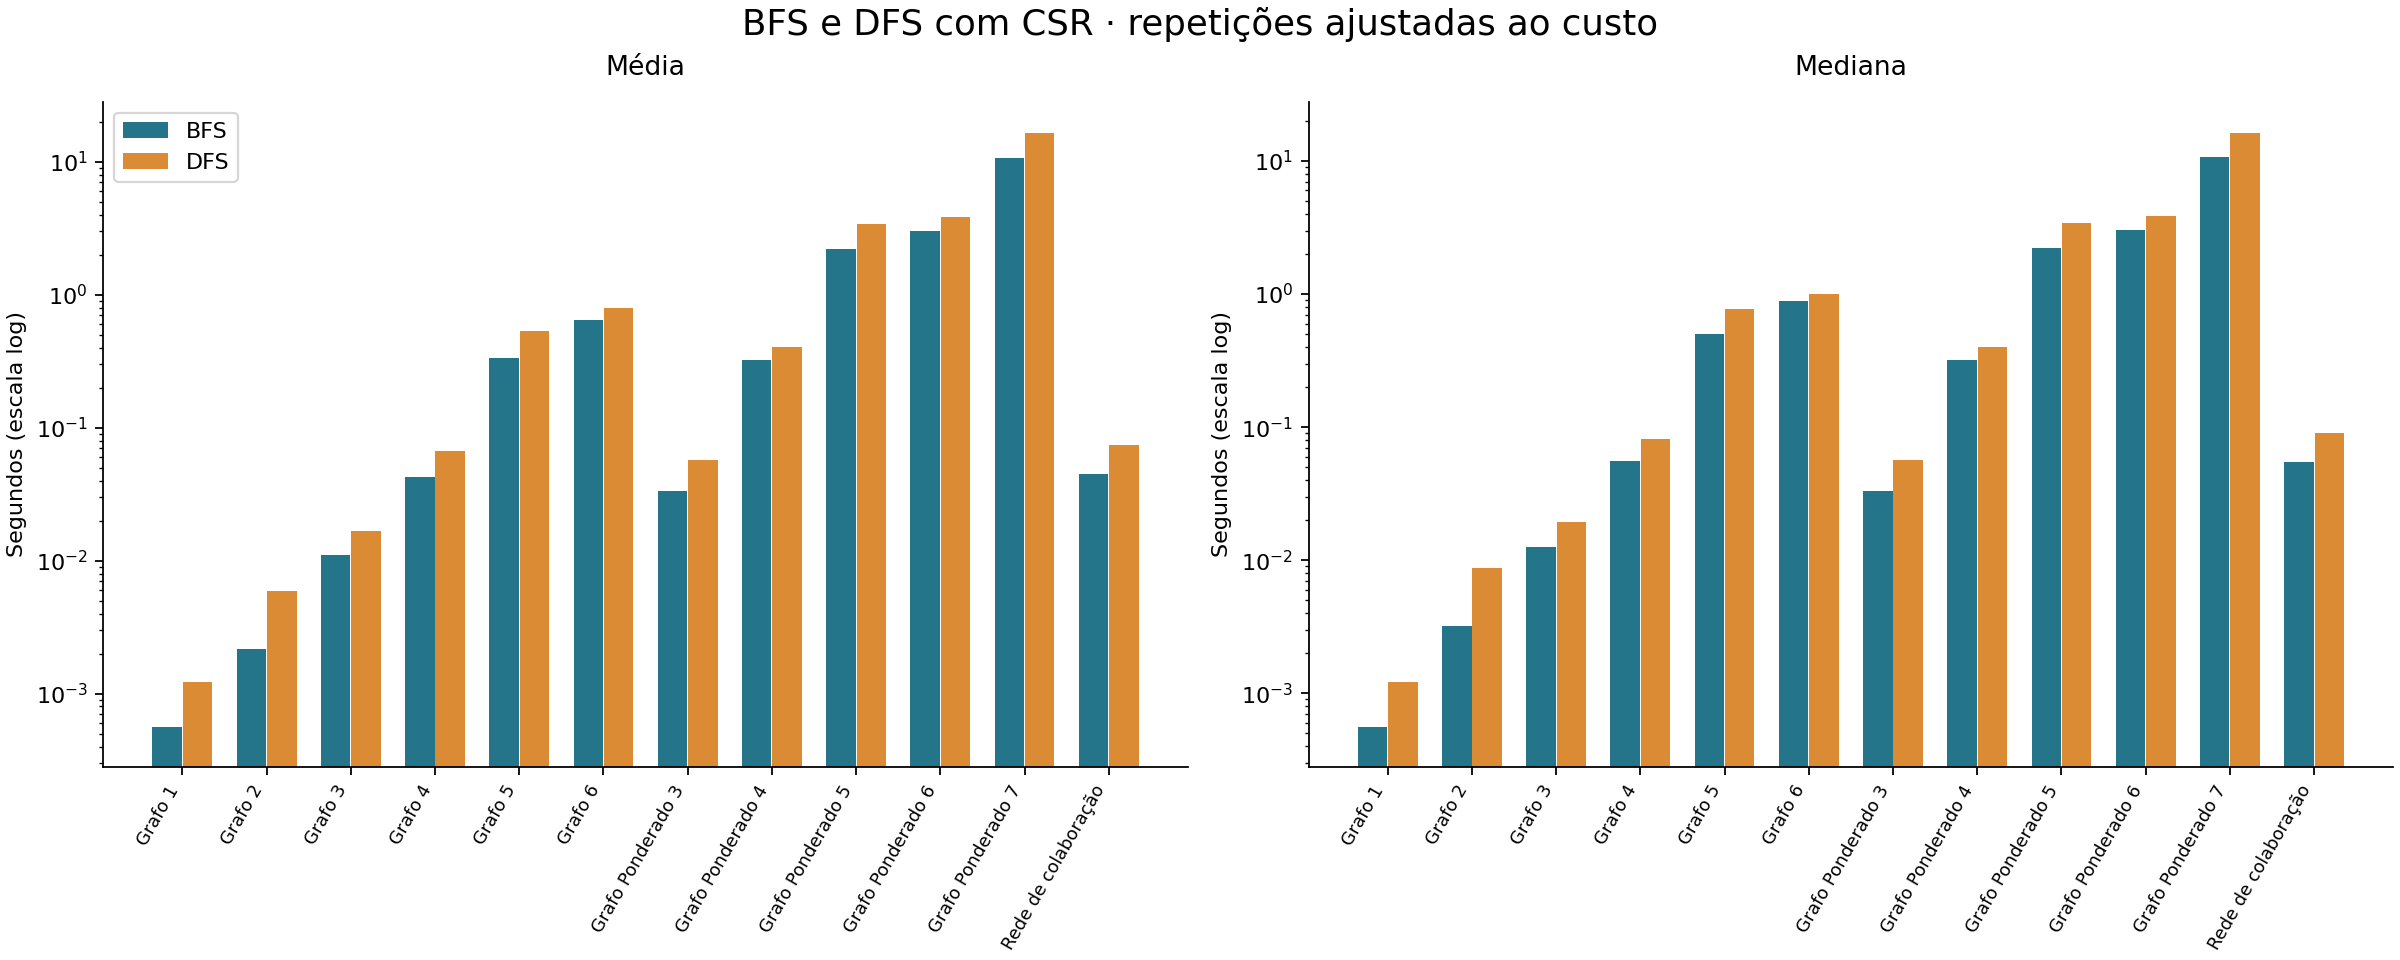
\includegraphics[width=\textwidth]{azure_traversals.png}\caption{BFS e DFS em CSR na nova rodada: médias e medianas, com contagens ajustadas ao custo.}\end{figure}
\begin{figure}[H]\centering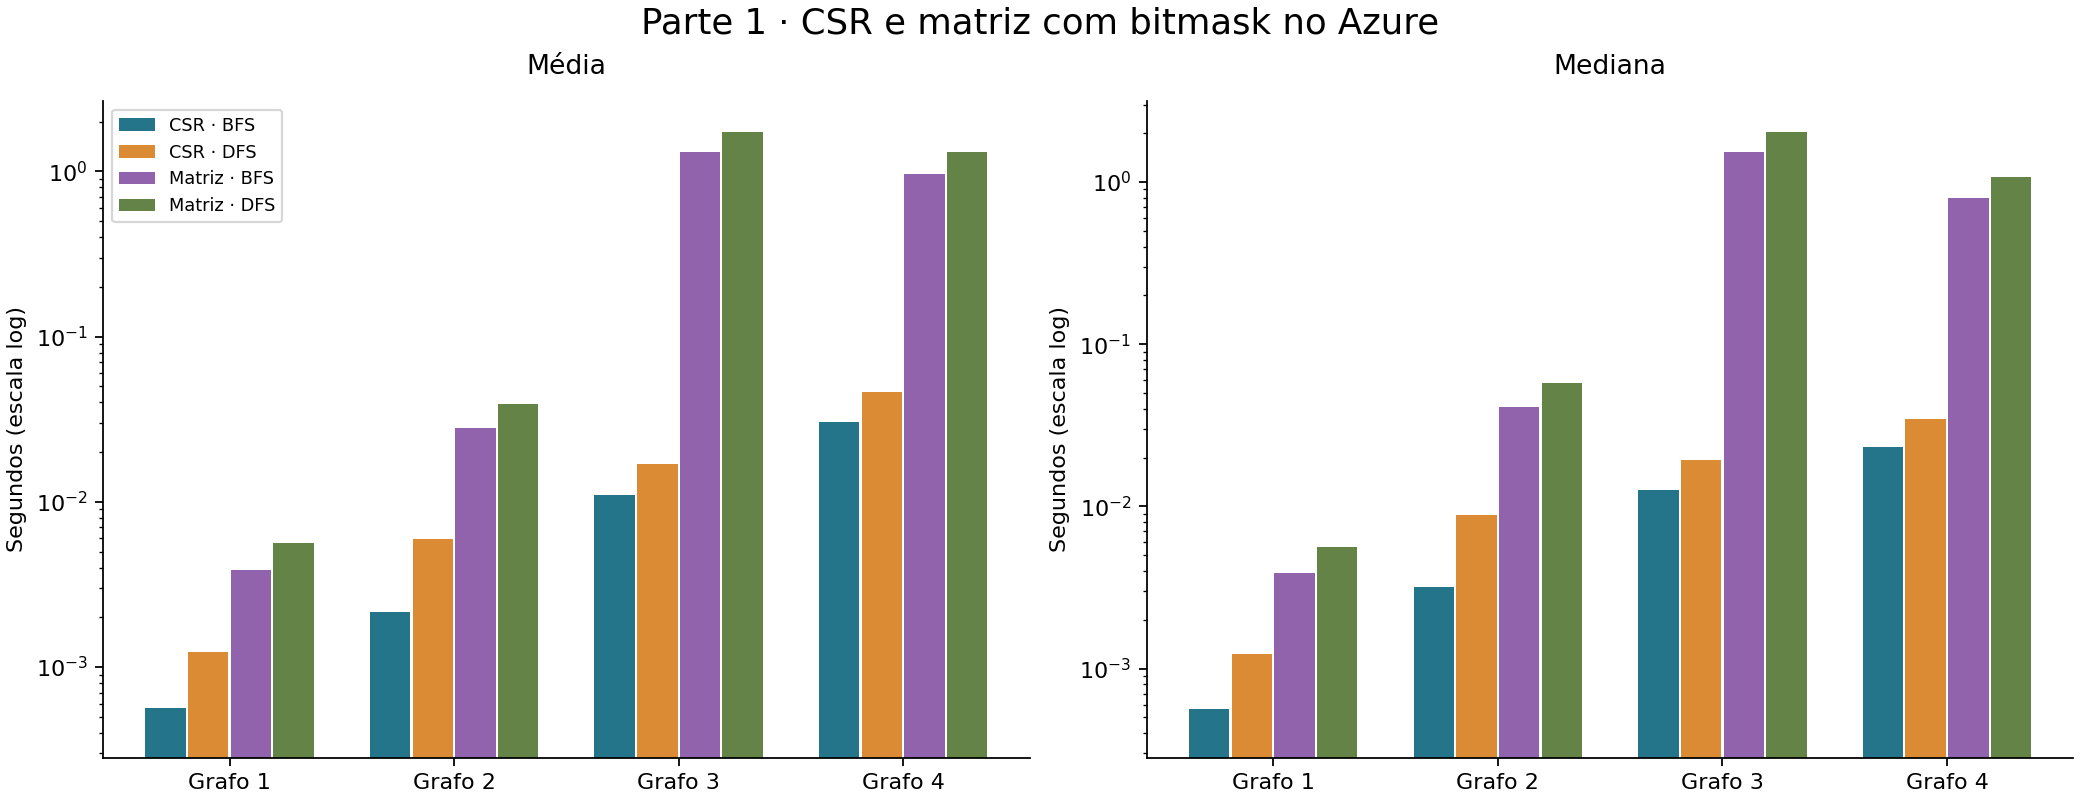
\includegraphics[width=\textwidth]{azure_traversals_matrix.png}\caption{Comparação pareada entre CSR e matriz com bitmask nos quatro grafos elegíveis.}\end{figure}
\begin{figure}[H]\centering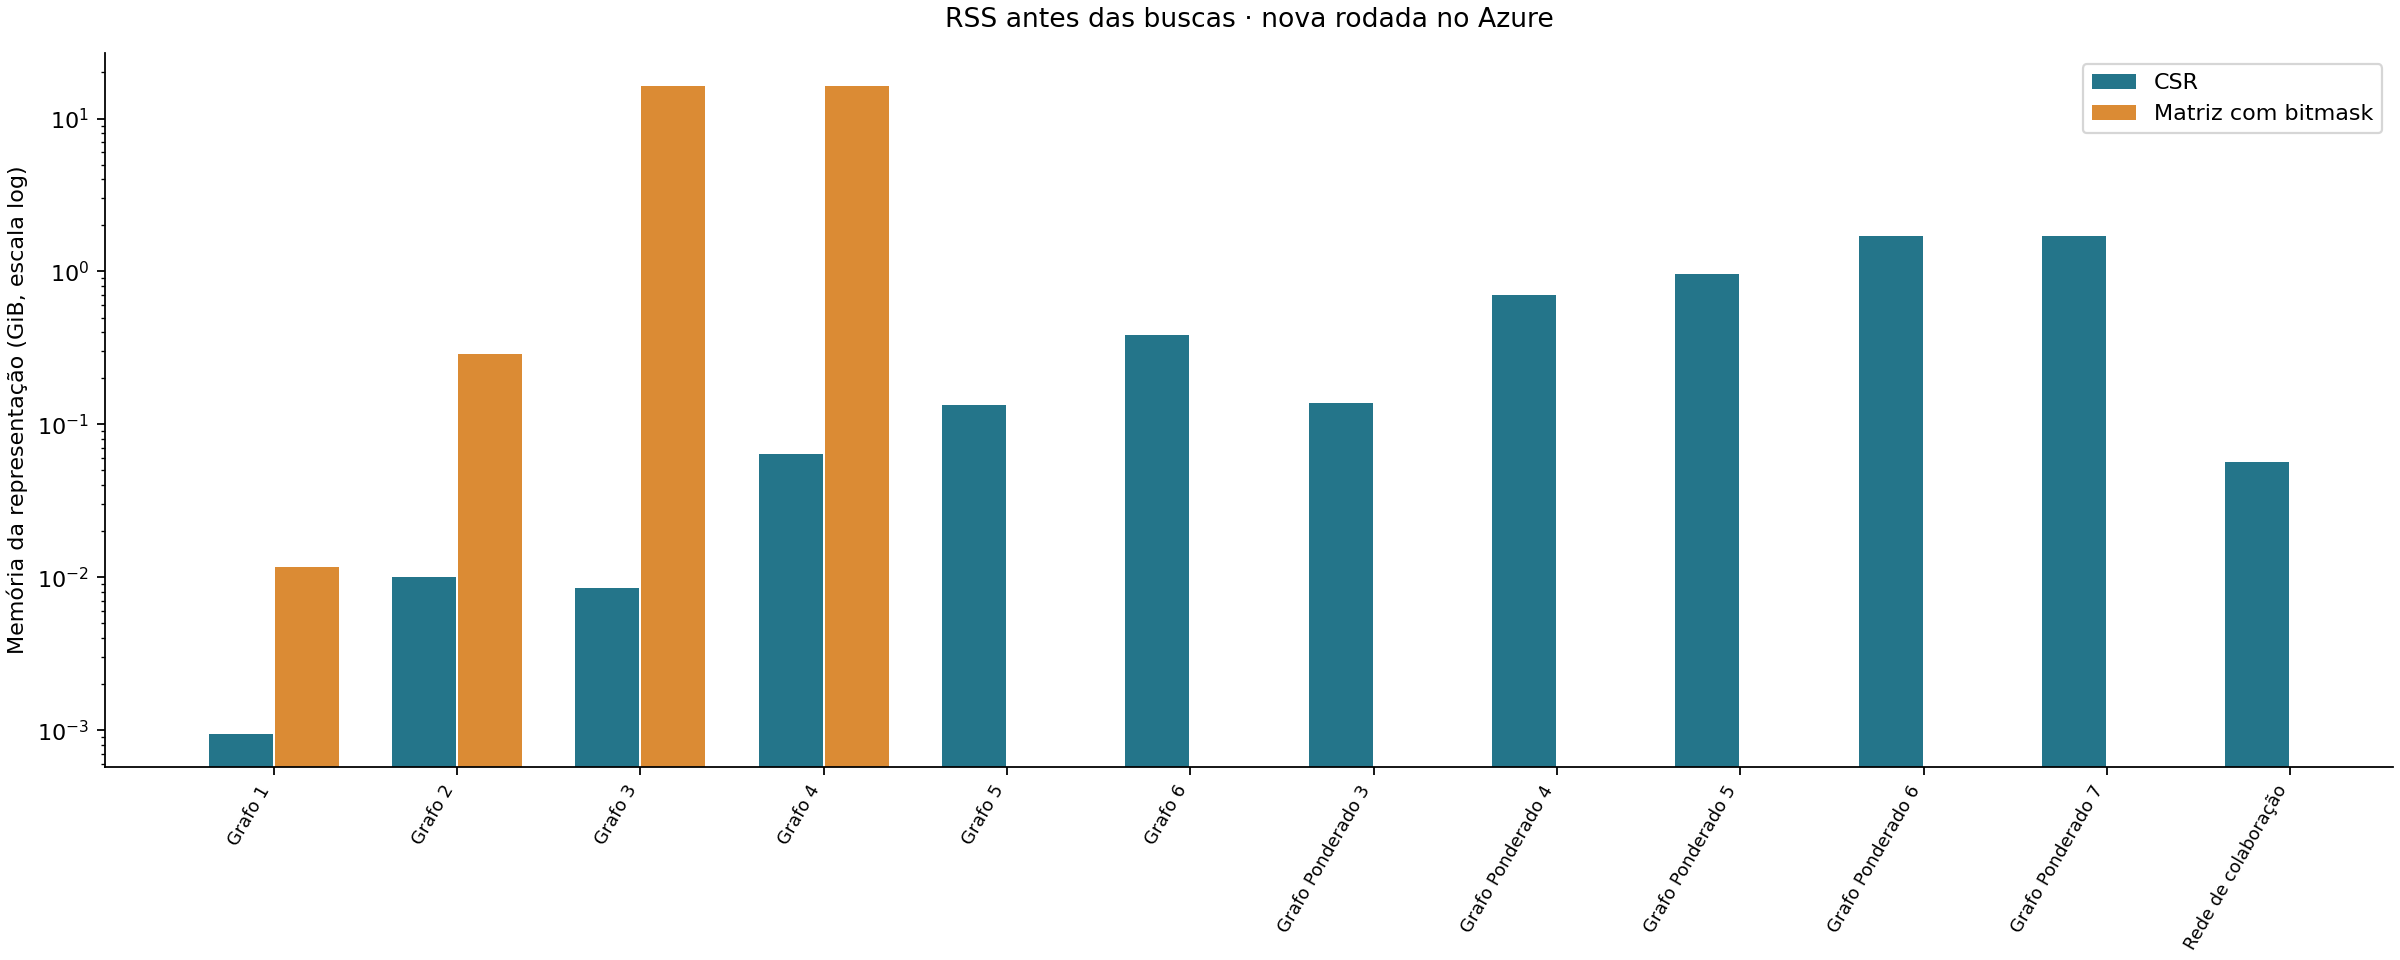
\includegraphics[width=\textwidth]{azure_traversals_memory.png}\caption{Memória das representações antes das buscas, medida em uma rodada distinta da de Dijkstra.}\end{figure}
\clearpage
\section{Compatibilidade e revisão das interpretações da Parte 1}
O relatório anterior é a referência de organização e de perguntas analíticas, não uma hipótese de que as representações permaneceram iguais. Três ajustes são necessários: (i) os laços agora são descartados e contados; (ii) o custo de inicializar vetores globais aparece mesmo em uma componente pequena; (iii) a bitmask muda constantes, memória e a forma de listar vizinhos.
\par\smallskip\noindent\begin{minipage}{\textwidth}\centering
\begingroup\fontsize{9}{11}\selectfont
\setlength{\tabcolsep}{4pt}
\begin{tabular}{lrrrr}
\toprule
Grafo & Arestas na Parte 1 & Arestas válidas atuais & Laços descartados & Paralelas \\
\midrule
1 & \num{109977} & \num{109973} & \num{4} & \num{52} \\
2 & \num{1299794} & \num{1299729} & \num{65} & \num{1019} \\
3 & \num{765618} & \num{765617} & \num{1} & \num{2} \\
4 & \num{8187427} & \num{8187392} & \num{35} & \num{406} \\
5 & \num{13168928} & \num{13168921} & \num{7} & \num{10} \\
6 & \num{46469670} & \num{46469627} & \num{43} & \num{148} \\
\bottomrule
\end{tabular}
\endgroup
\captionof{table}{Reconciliação das contagens; os dados não foram silenciosamente substituídos.}
\end{minipage}\par\smallskip
\par\smallskip\noindent\begin{minipage}{\textwidth}\centering
\begingroup\fontsize{9}{11}\selectfont
\setlength{\tabcolsep}{4pt}
\begin{tabular}{lrrrrrr}
\toprule
Grafo & $N$ & Comp. & Maior & Menor & Grau médio & Mediana \\
\midrule
1 & \num{10000} & \num{1} & \num{10000} & \num{10000} & \num{21.9946} & \num{22} \\
2 & \num{49948} & \num{10} & \num{25000} & \num{48} & \num{52.0433} & \num{55} \\
3 & \num{375000} & \num{2} & \num{250000} & \num{125000} & \num{4.08329} & \num{4} \\
4 & \num{375000} & \num{2} & \num{250000} & \num{125000} & \num{43.6661} & \num{47} \\
5 & \num{4843750} & \num{5} & \num{2500000} & \num{156250} & \num{5.43749} & \num{5} \\
6 & \num{4843750} & \num{5} & \num{2500000} & \num{156250} & \num{19.1875} & \num{20} \\
\bottomrule
\end{tabular}
\endgroup
\end{minipage}\par\smallskip

A exploração em CSR custa $O(N+N_c+M_c)$, pois os vetores são dimensionados para todo o grafo. A DFS marca ao remover da pilha e pode manter cópias pendentes de um mesmo vértice; a BFS marca ao inserir na fila. A profundidade da DFS não é distância mínima. Na bitmask, listar vizinhos varre palavras de 64 bits e enumera os bits presentes, em vez de testar cada célula individualmente.

Dupla varredura fornece um limite inferior na maior componente, em arestas e ignorando pesos. O limite 4 no Grafo 1 é compatível com o diâmetro 5 informado anteriormente. No Grafo 5, os valores 11 (anterior) e 12 (atual) são aproximações: origens e escopo podem alterar o limite obtido. Maior densidade global não garante menor diâmetro em grafos distintos.
\par\smallskip\noindent\begin{minipage}{\textwidth}\centering
\begingroup\fontsize{8.8}{11}\selectfont
\setlength{\tabcolsep}{4pt}
\begin{tabular}{lrr}
\toprule
Grafo & Exato, máximo nas componentes & Limite inferior, maior componente \\
\midrule
Grafo 1 & -- & \num{4} \\
Grafo 2 & -- & \num{3} \\
Grafo 3 & -- & \num{14} \\
Grafo 4 & -- & \num{4} \\
Grafo 5 & -- & \num{12} \\
Grafo 6 & -- & \num{6} \\
Grafo Ponderado 3 & -- & \num{3} \\
Grafo Ponderado 4 & -- & \num{5} \\
Grafo Ponderado 5 & -- & \num{11} \\
Grafo Ponderado 6 & -- & \num{8} \\
Grafo Ponderado 7 & -- & \num{75} \\
Rede de colaboração & -- & \num{23} \\
\bottomrule
\end{tabular}
\endgroup
\end{minipage}\par\smallskip
\clearpage\section{Distribuições e visualizações das redes}

As frequências de graus e tamanhos de componentes usam todos os dados exportados e são exibidas apenas por pontos, sem ligá-los. Histograma de pesos é uma agregação por intervalos de uma variável numérica real; não é a frequência exata de cada peso distinto. A função acumulada complementar do grau indica a fração de vértices com grau pelo menos igual ao valor do eixo horizontal.
\begin{figure}[H]\centering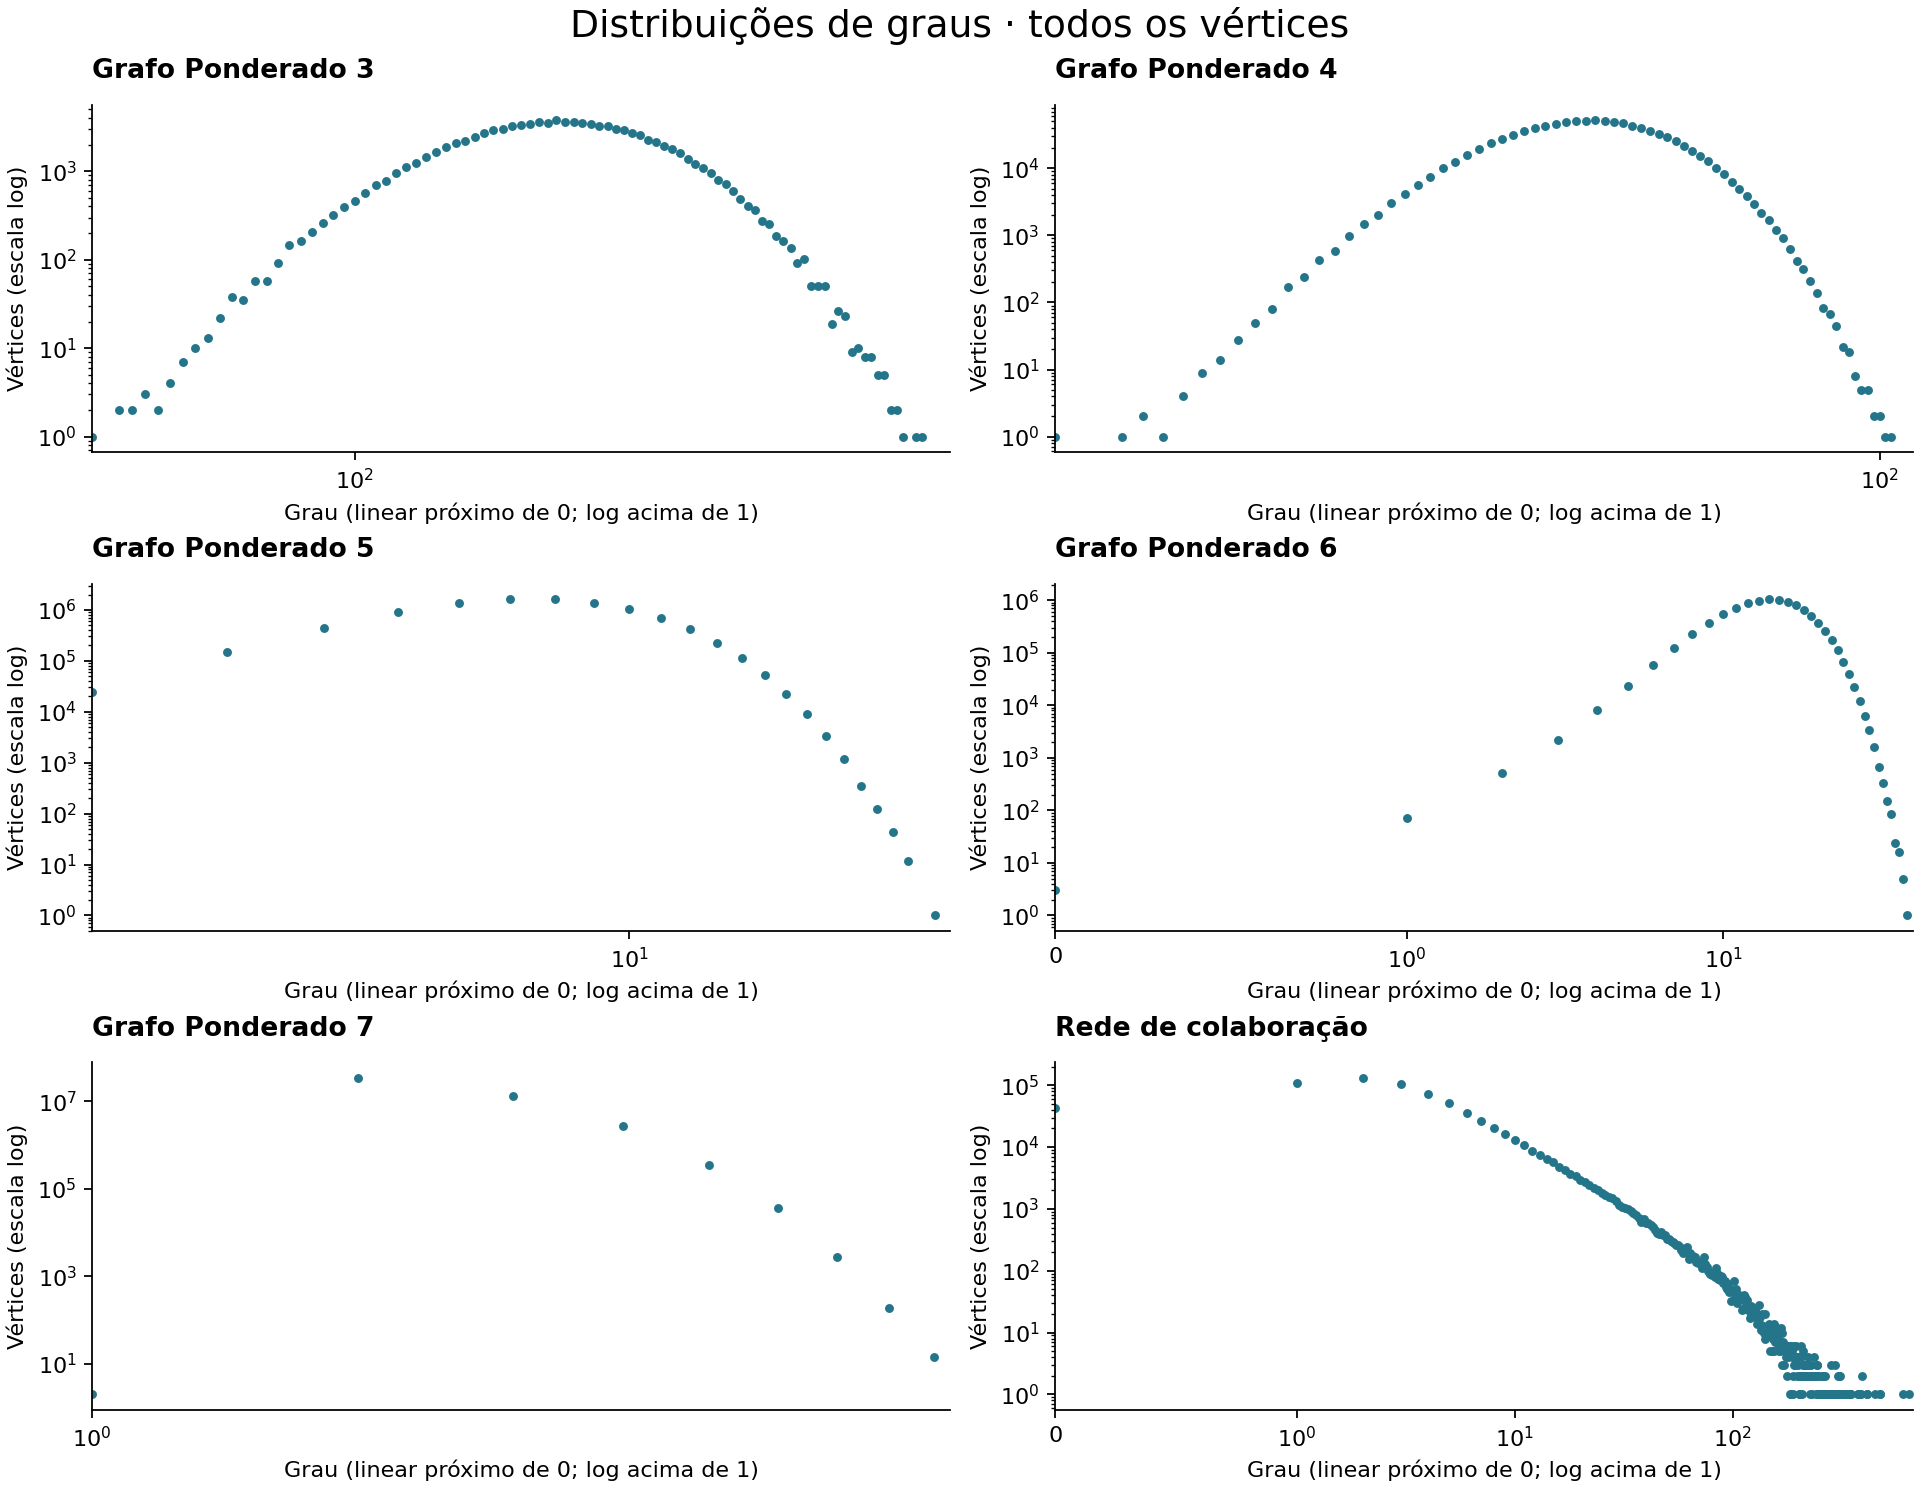
\includegraphics[width=\textwidth]{parte2/degree_frequencies.png}\caption{Frequências exatas de grau nos grafos ponderados; cada marcador corresponde a um grau observado.}\end{figure}
\clearpage
\begin{figure}[H]\centering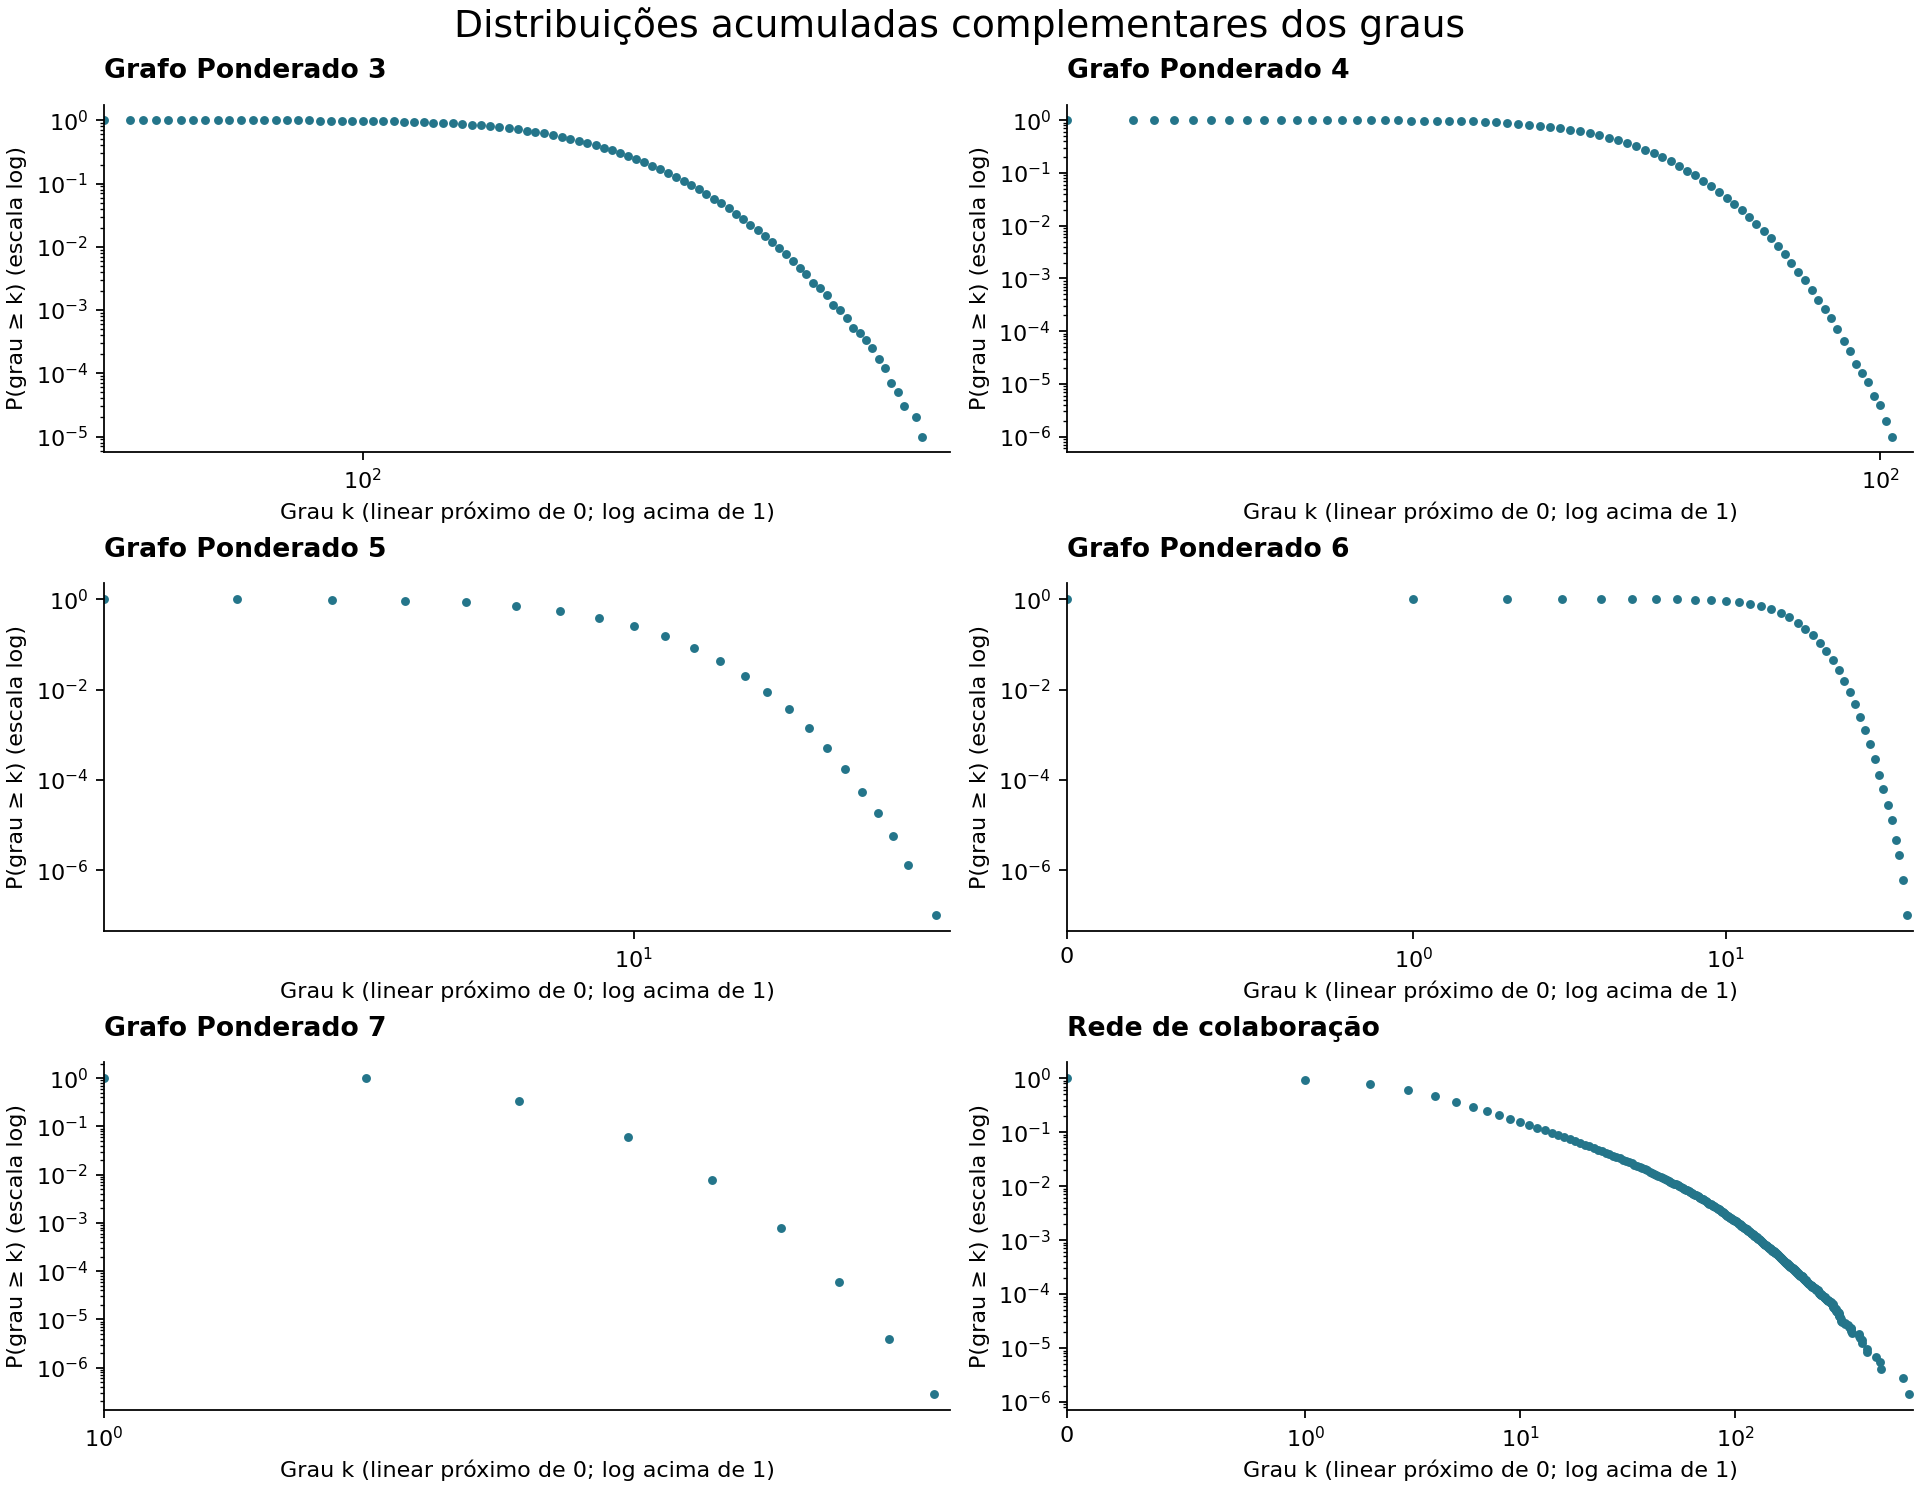
\includegraphics[width=\textwidth]{parte2/degree_tails.png}\caption{Distribuições acumuladas complementares dos graus; dados discretos sem linhas de ligação.}\end{figure}
\clearpage
\begin{figure}[H]\centering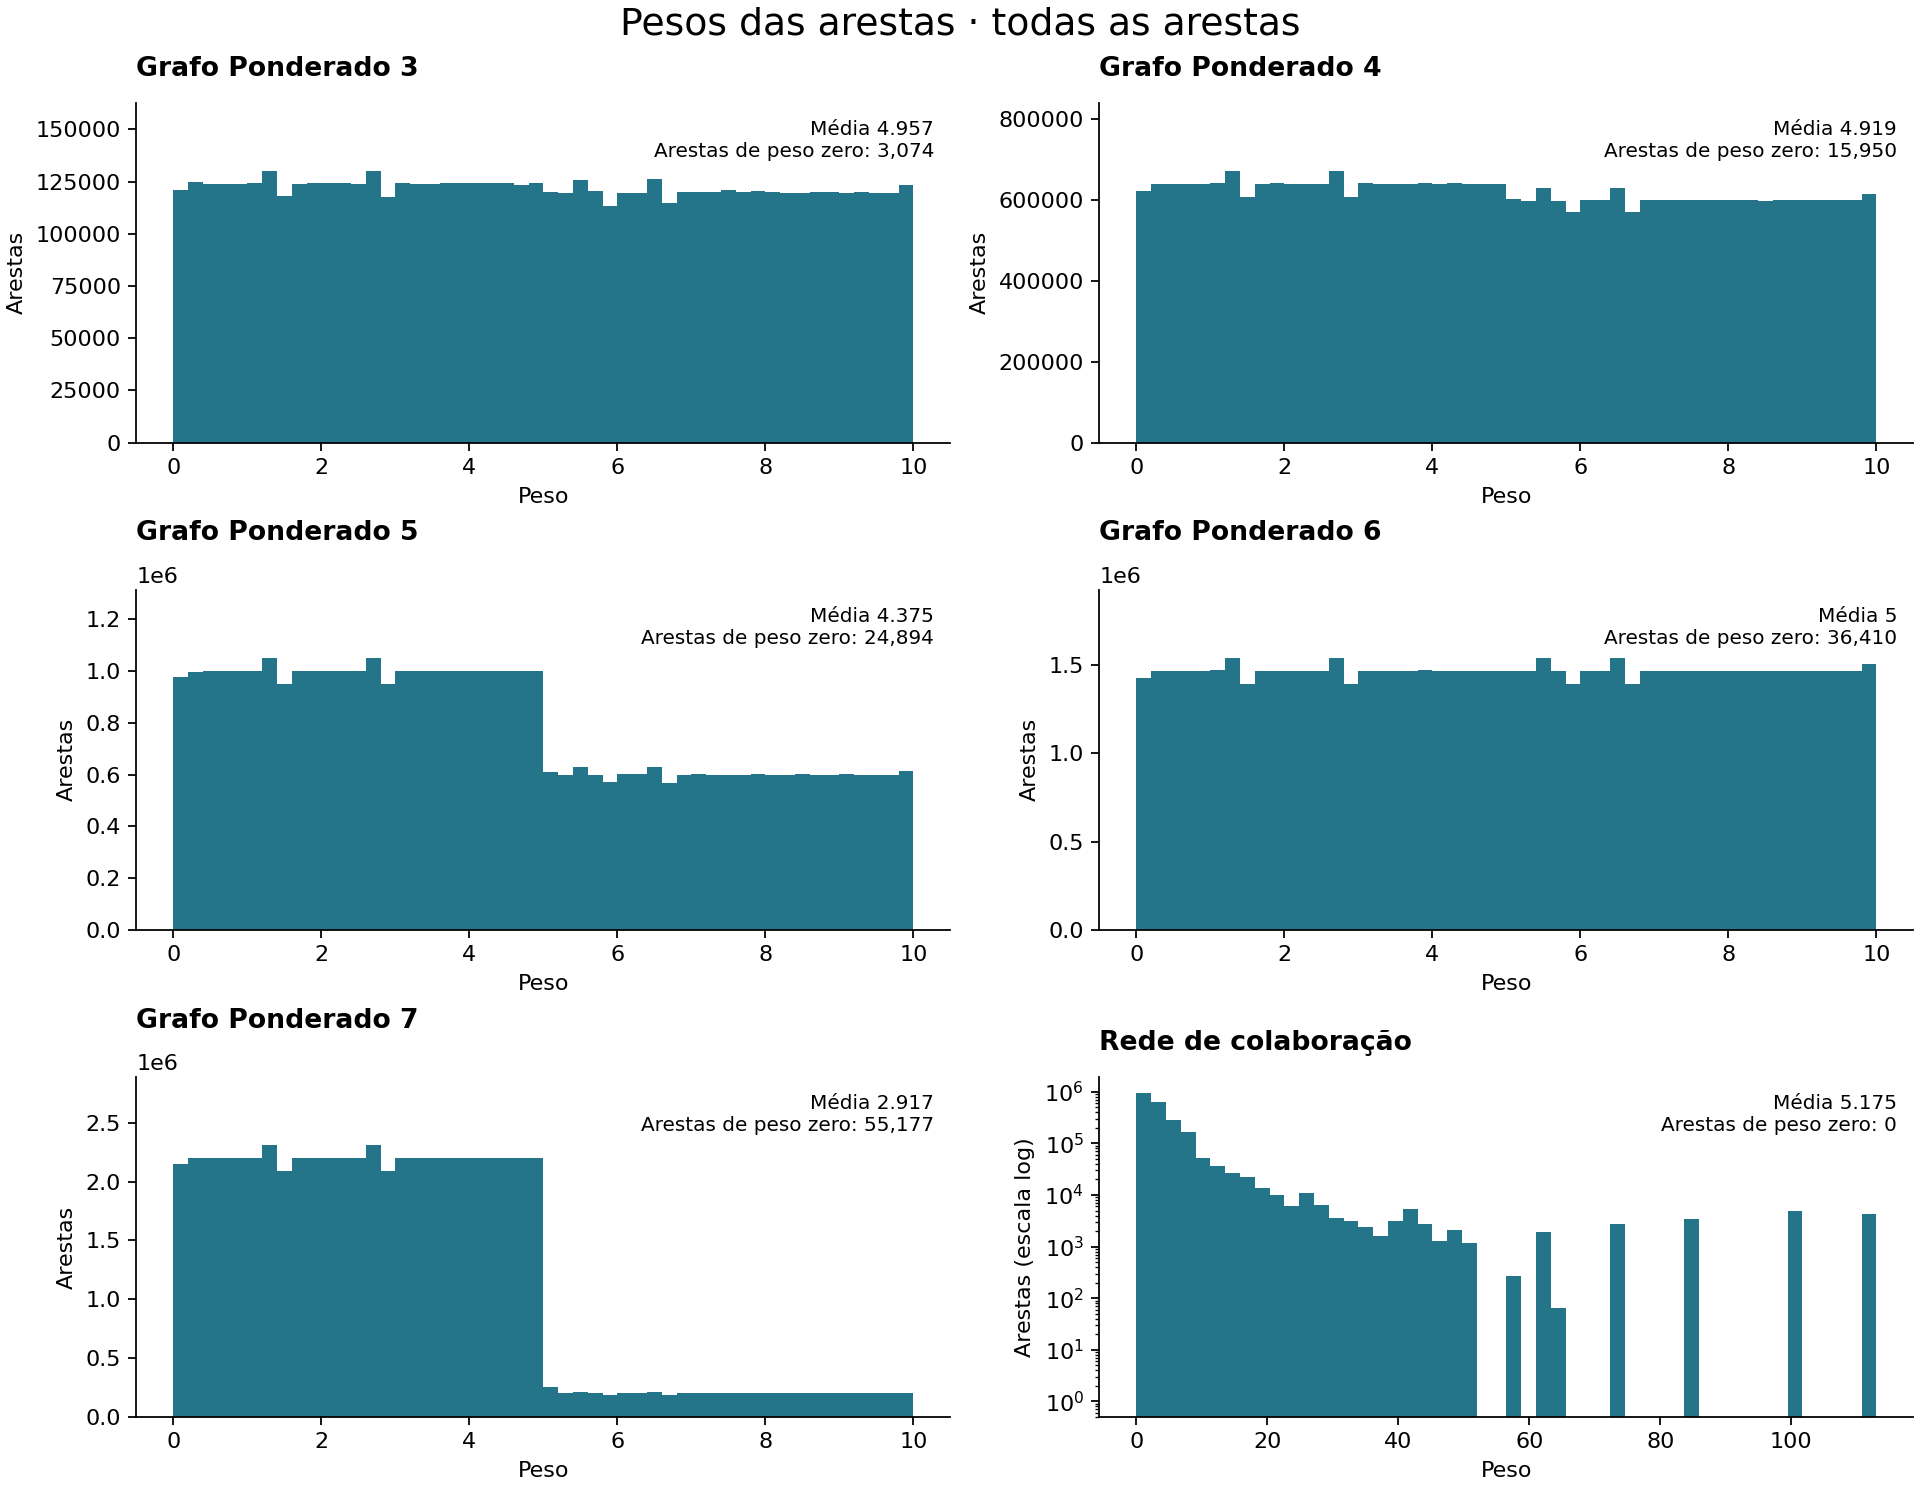
\includegraphics[width=\textwidth]{parte2/weight_distributions.png}\caption{Distribuições dos pesos em intervalos; a escala dos pesos muda entre grafos.}\end{figure}
\clearpage
\begin{figure}[H]\centering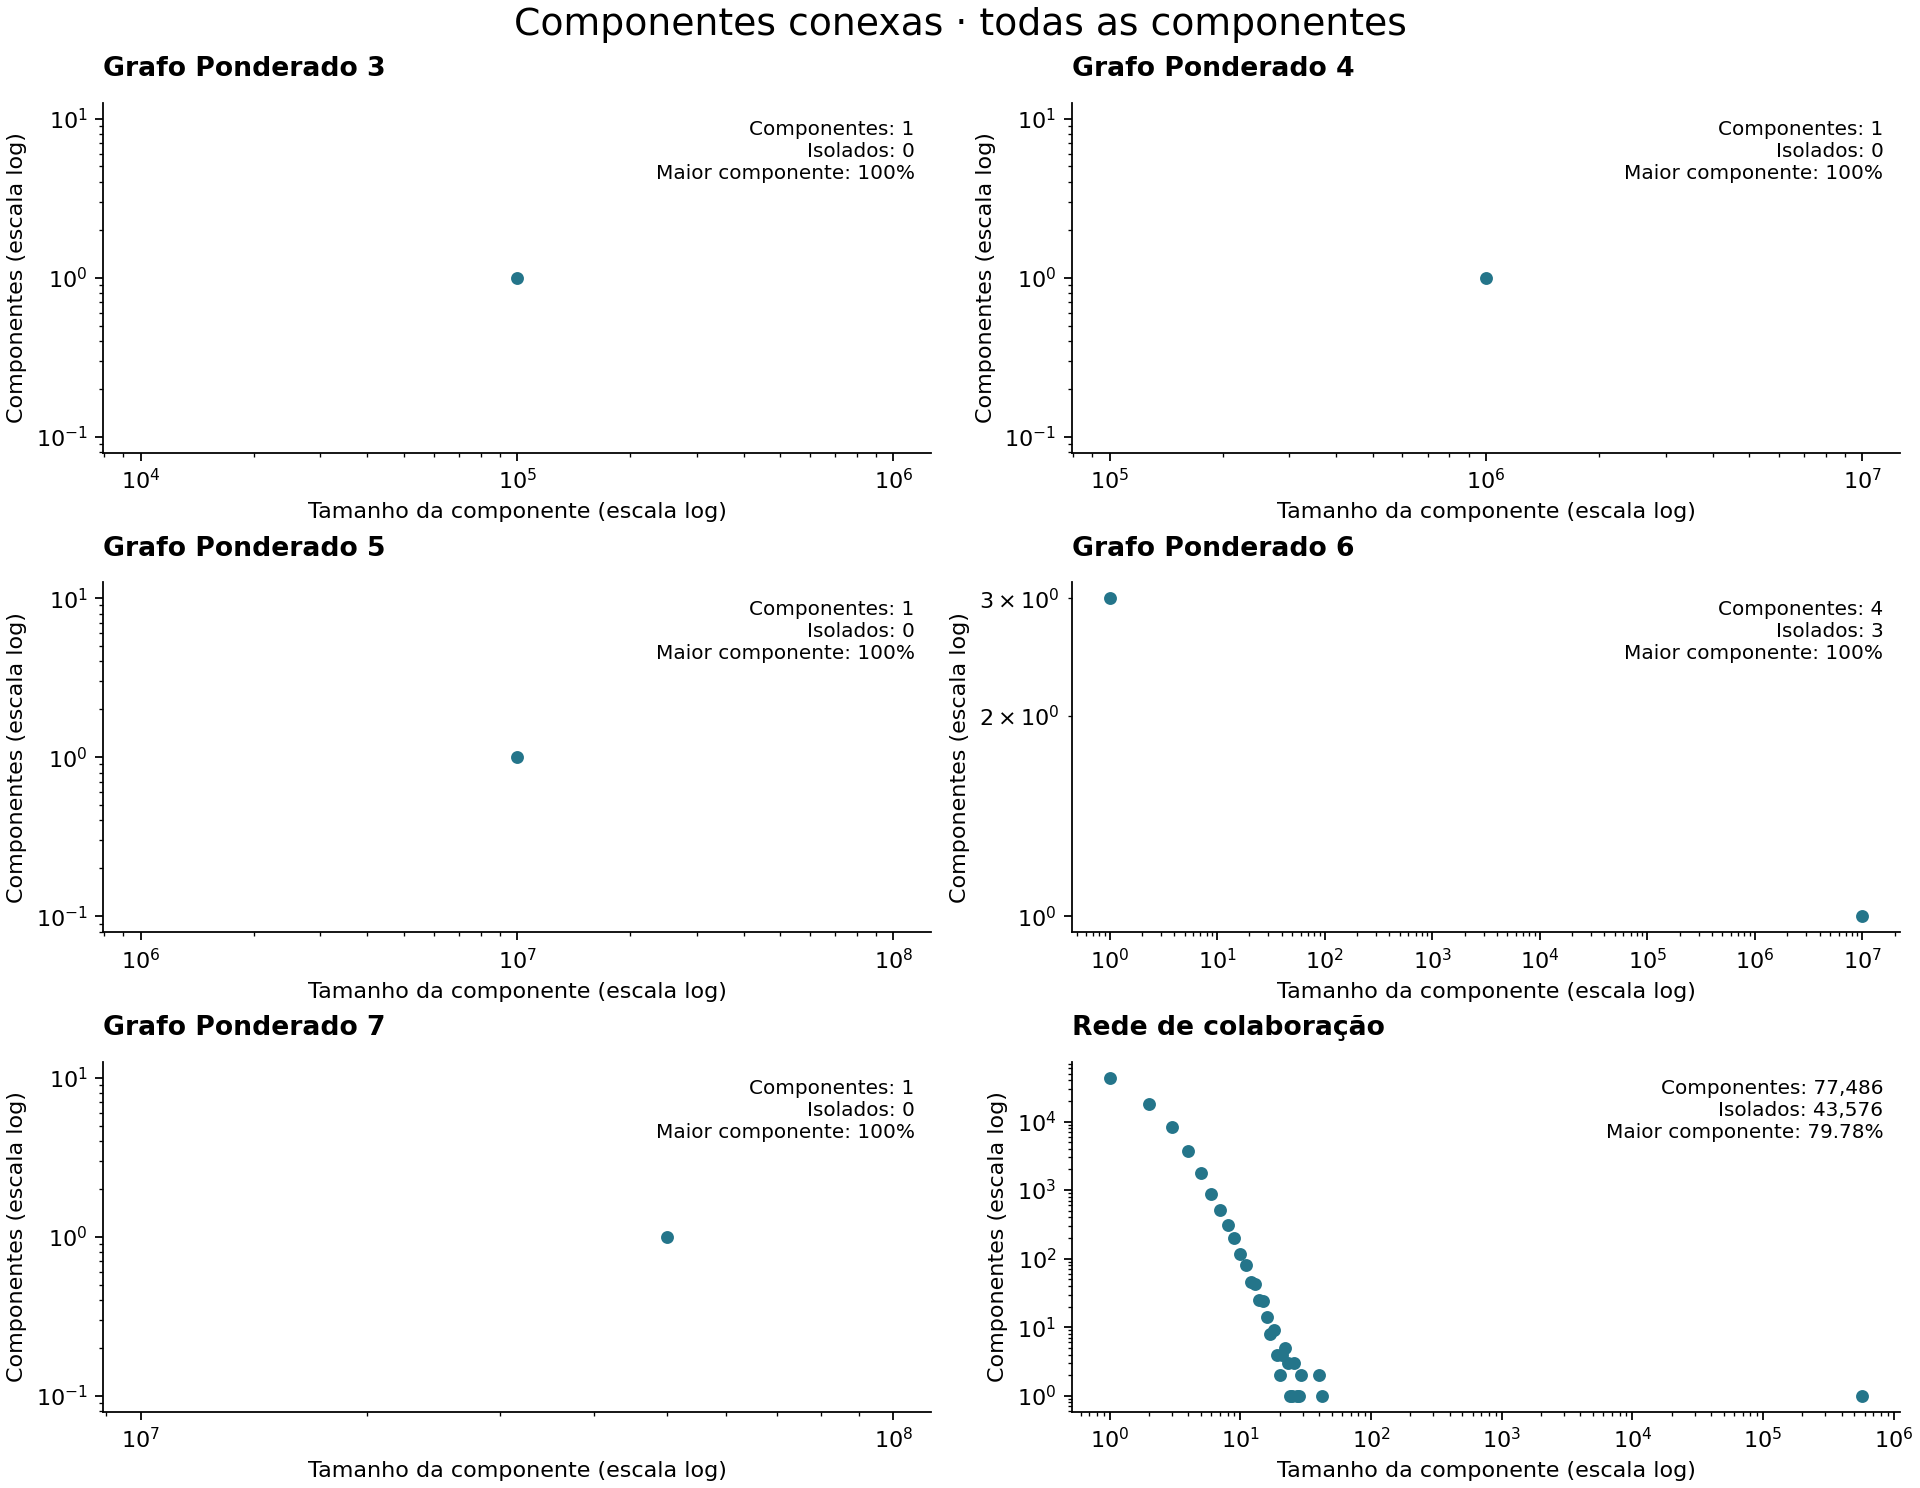
\includegraphics[width=\textwidth]{parte2/component_sizes.png}\caption{Tamanhos e multiplicidades das componentes, representados por pontos.}\end{figure}
\clearpage
\begin{figure}[H]\centering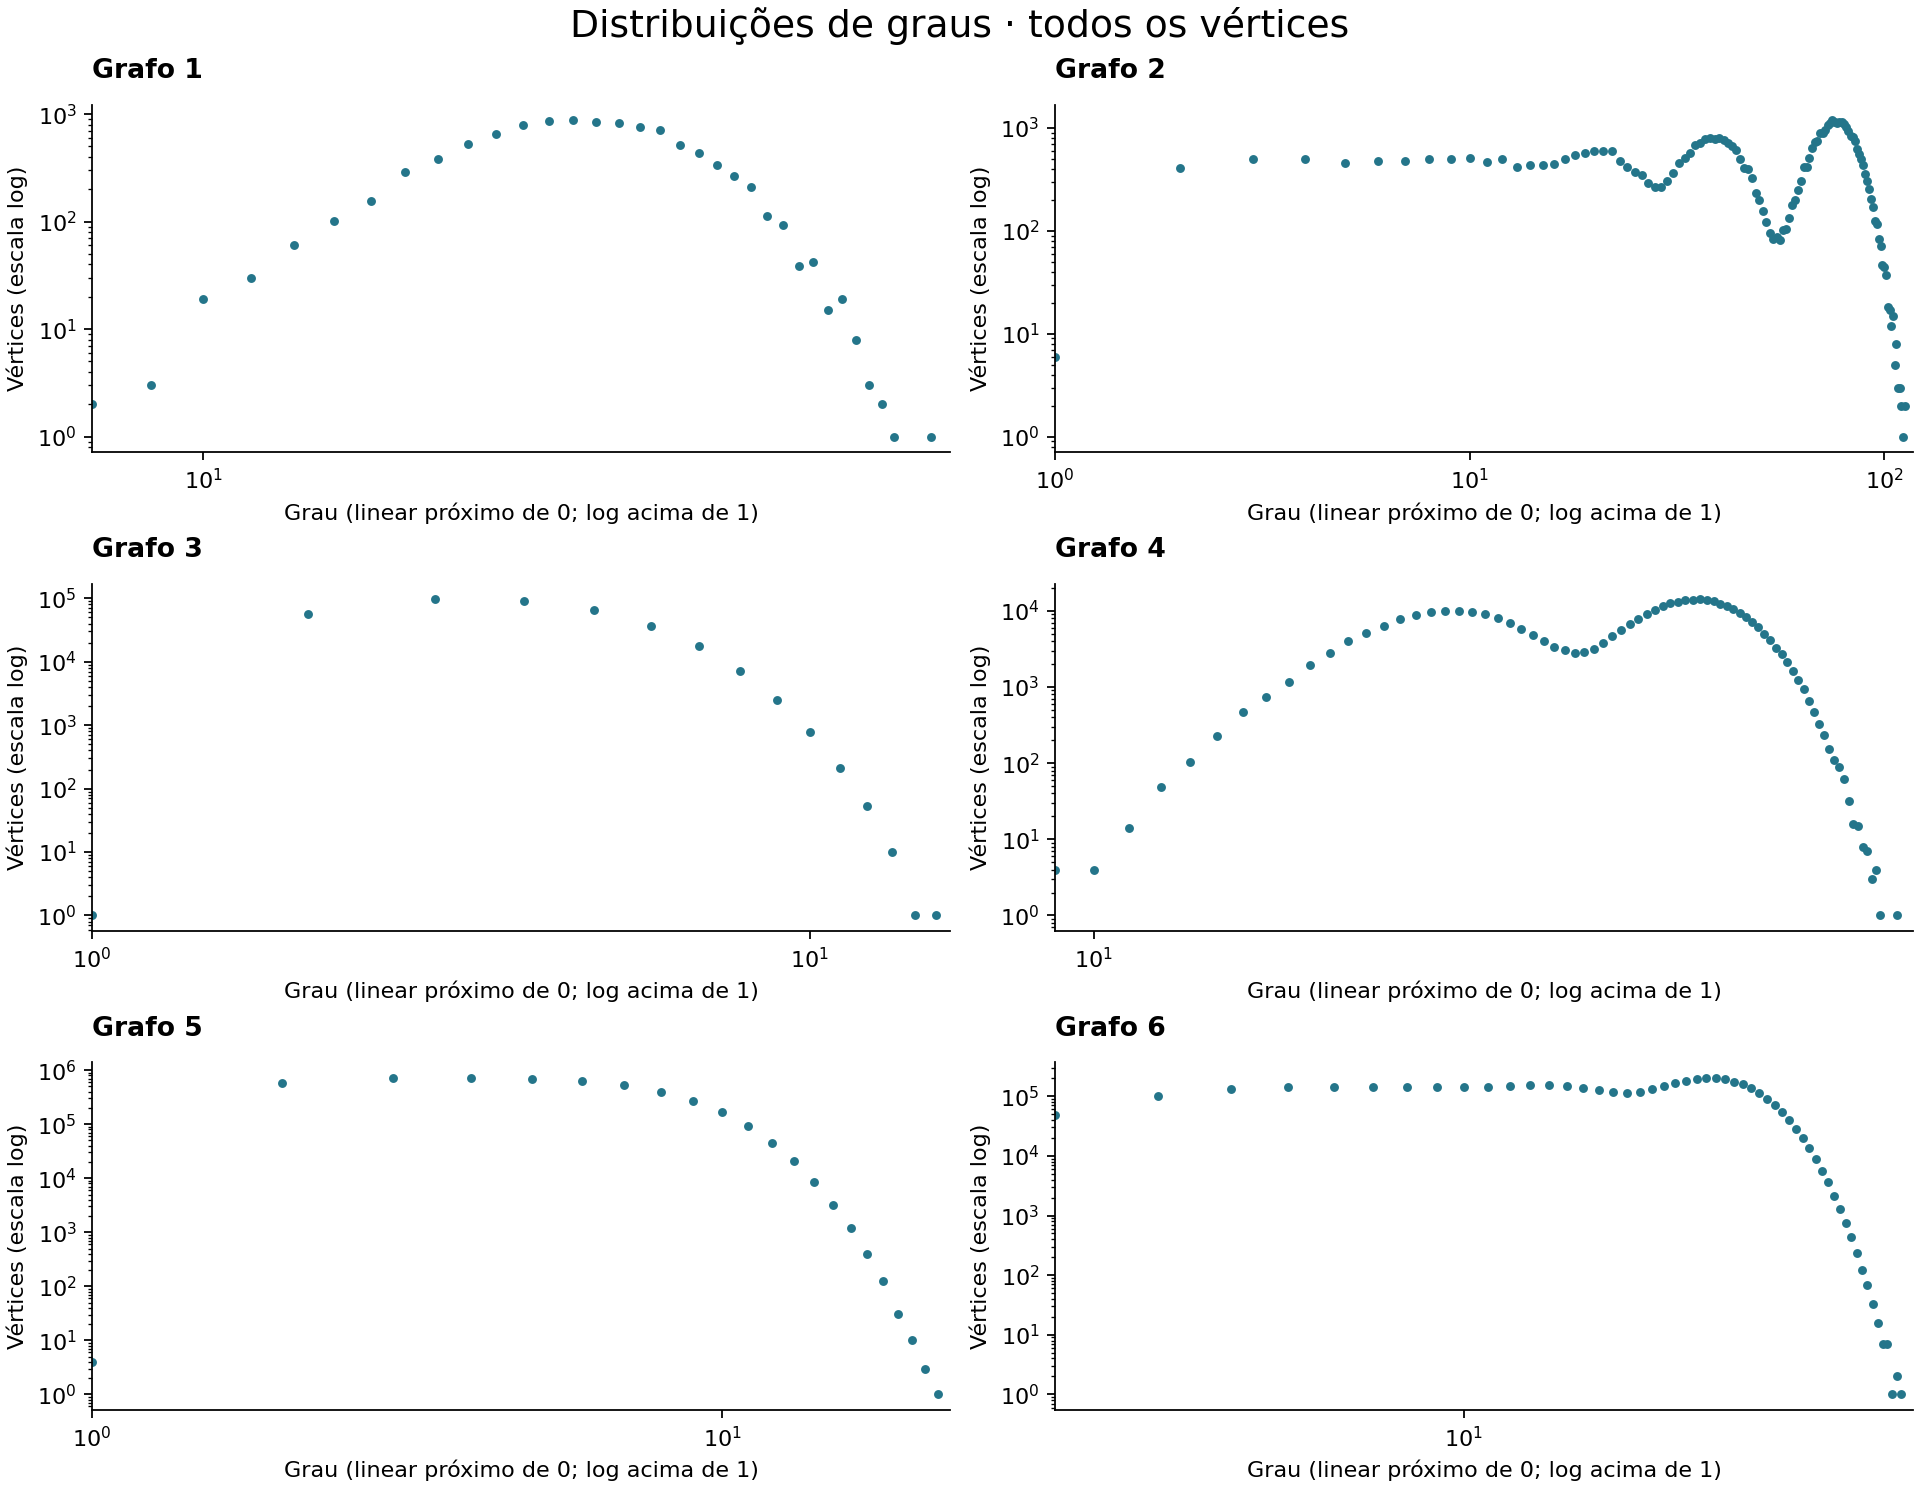
\includegraphics[width=\textwidth]{parte1/degree_frequencies.png}\caption{Frequências exatas de grau dos seis grafos não ponderados.}\end{figure}
\clearpage
\begin{figure}[H]\centering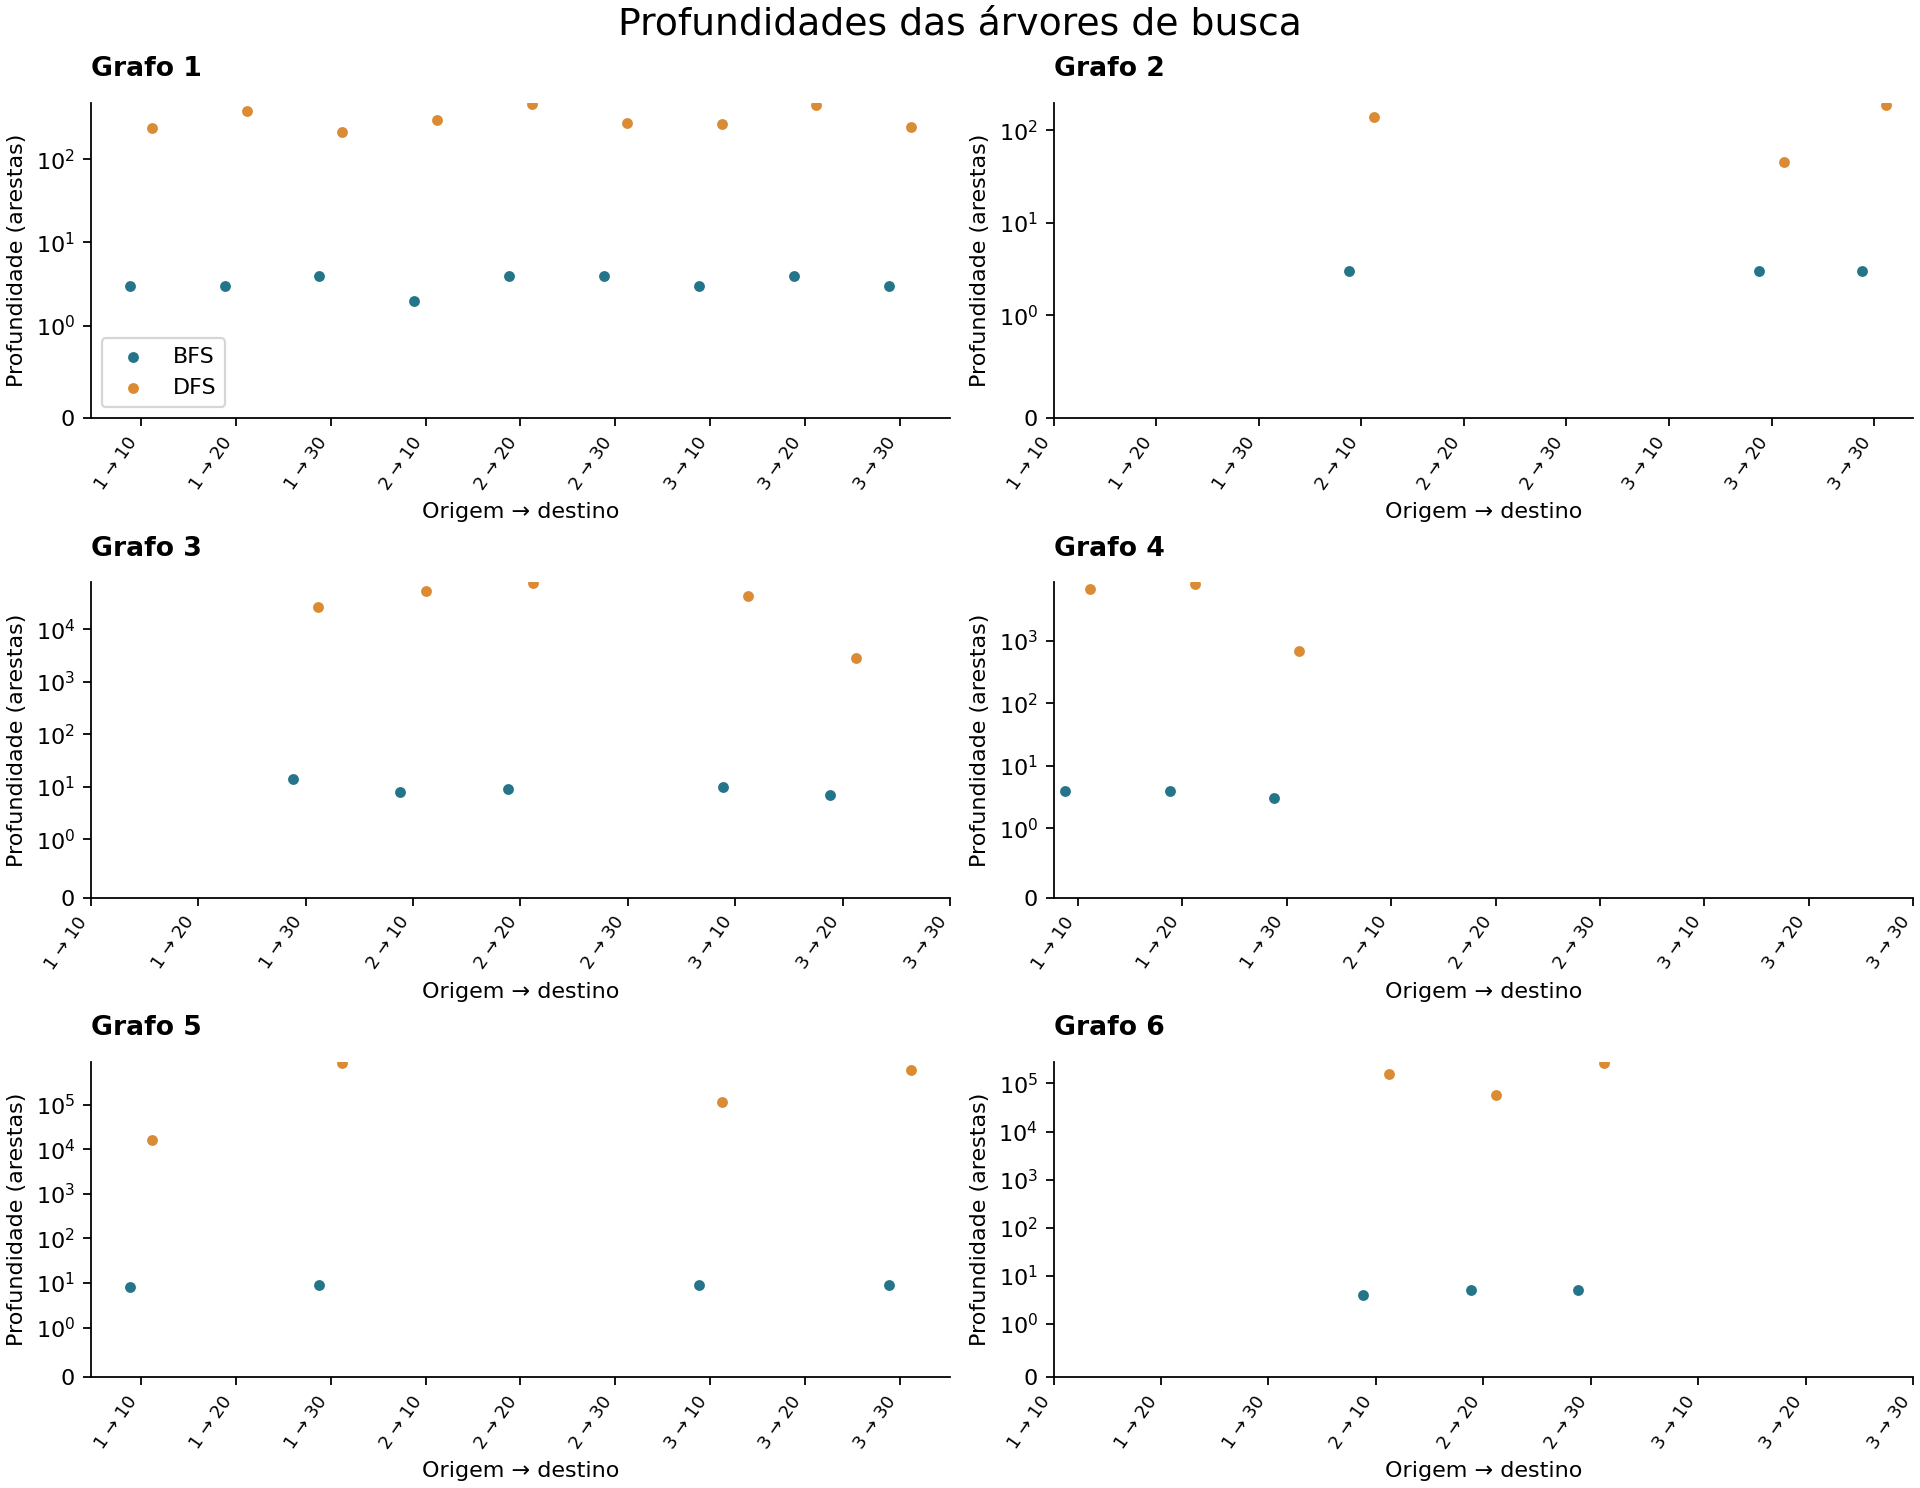
\includegraphics[width=\textwidth]{parte1/search_depths.png}\caption{Comparação entre níveis de BFS e profundidades de DFS nos estudos de caso da Parte 1.}\end{figure}
\clearpage
\subsection{Amostras de rede: significado e limites}
Cada figura mostra uma amostra distribuída e outra de vizinhança, limitadas a 1.000 vértices e 4.000 arestas exportadas. Os detalhes de seleção estão no CSV de metadados de cada amostra; o desenho usa semente 2025 e 45 iterações. As posições são ilustrativas e não codificam distância geográfica, distância ponderada ou importância causal. O peso da aresta não determina o comprimento visual.

A escala do vértice representa seu grau no grafo original, não apenas na amostra. Um vértice sem ligação desenhada pode ter vizinhos fora da seleção ou arestas omitidas pelo limite; somente a marcação de isolado indica grau zero no grafo original. As amostras não estimam número de componentes nem diâmetro do grafo inteiro. Os valores globais vêm das tabelas e distribuições exatas.
\begin{figure}[H]\centering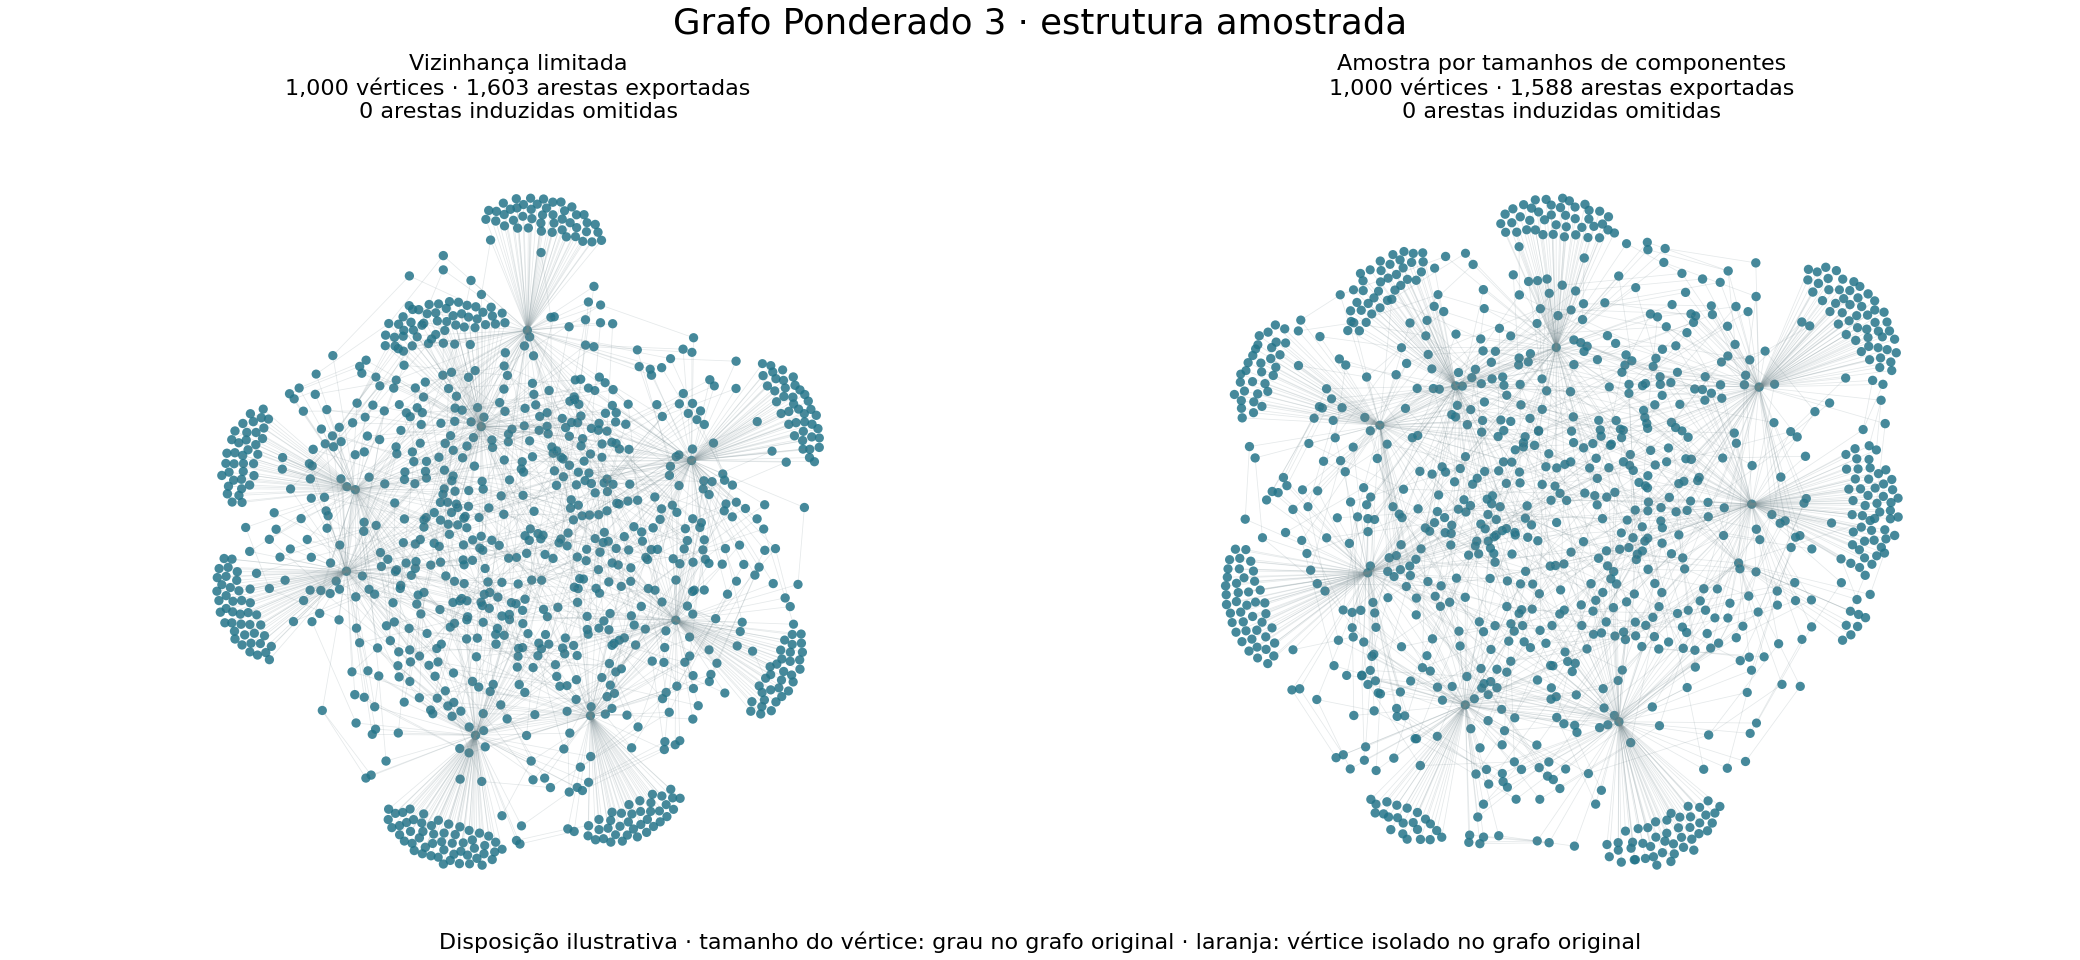
\includegraphics[width=\textwidth]{network_grafo_W_3.png}\caption{Estrutura amostrada de Grafo Ponderado 3. Os dois painéis não representam o grafo inteiro.}\end{figure}
\begin{figure}[H]\centering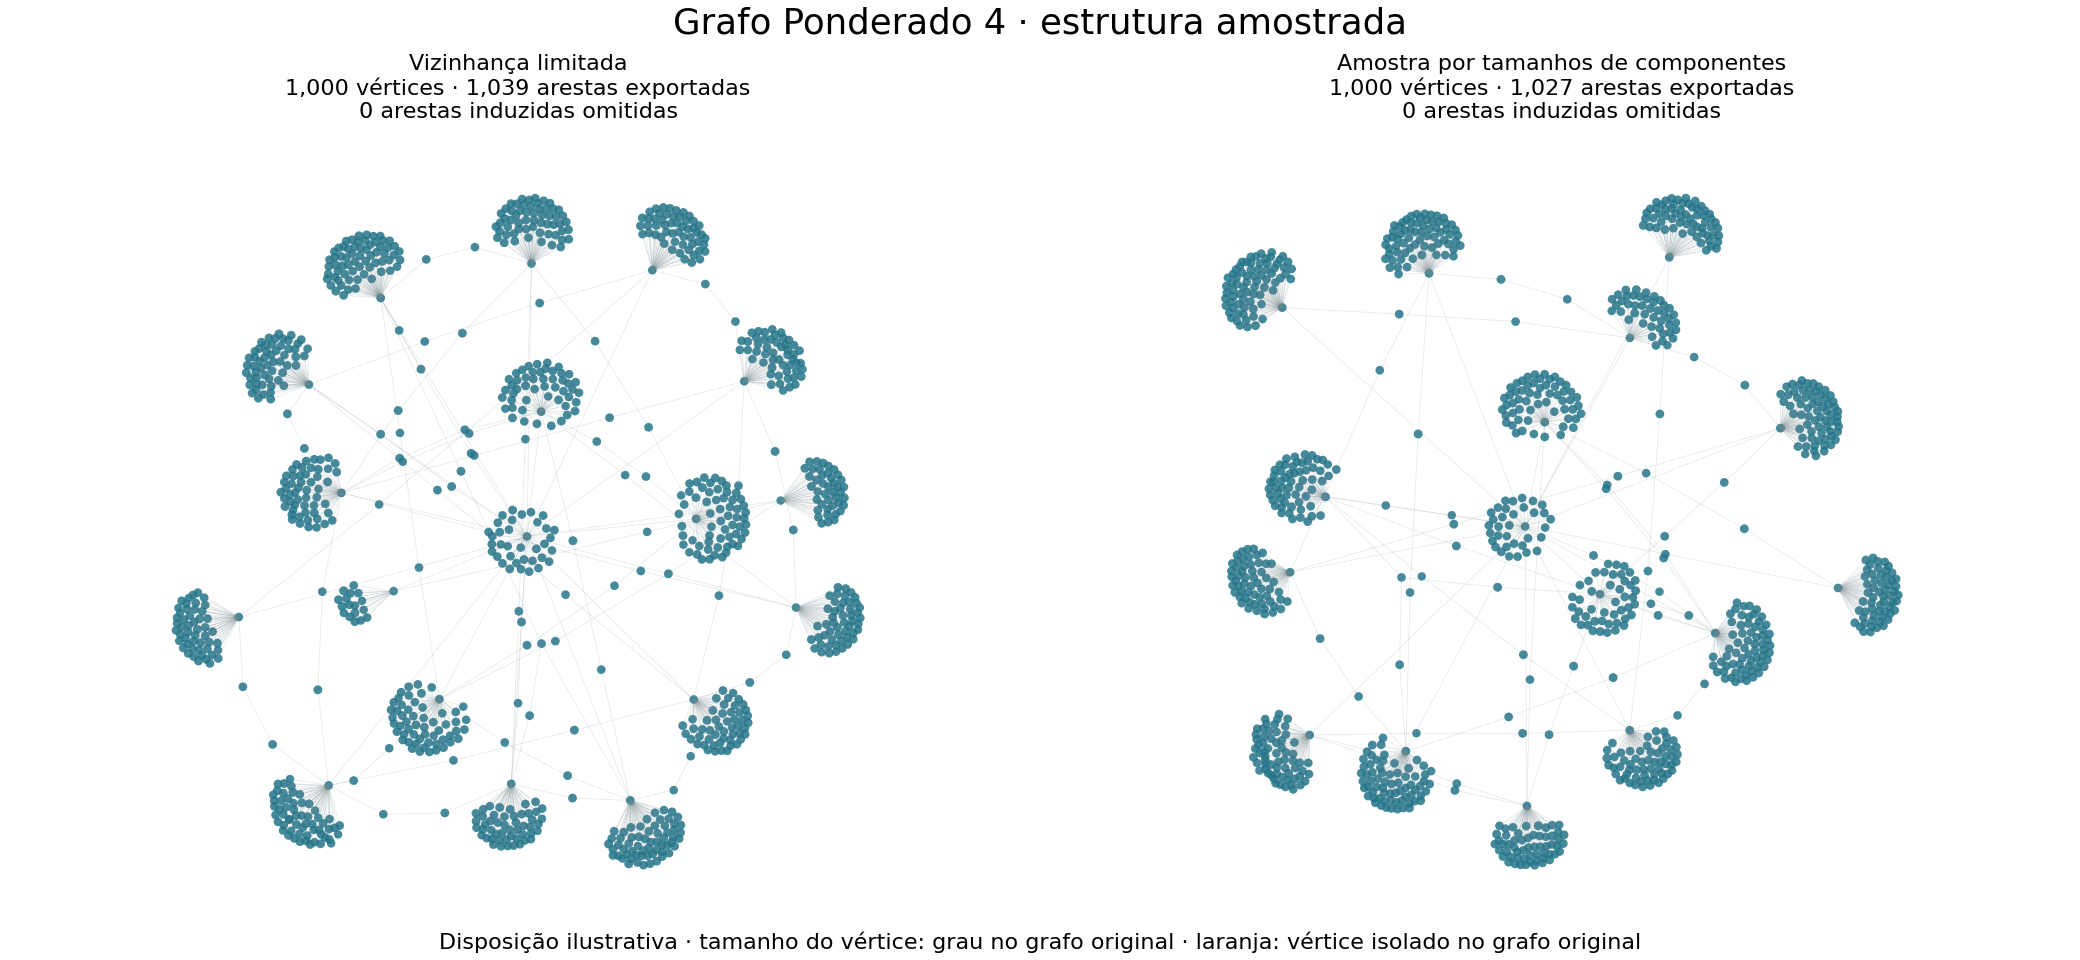
\includegraphics[width=\textwidth]{network_grafo_W_4.png}\caption{Estrutura amostrada de Grafo Ponderado 4. Os dois painéis não representam o grafo inteiro.}\end{figure}
\begin{figure}[H]\centering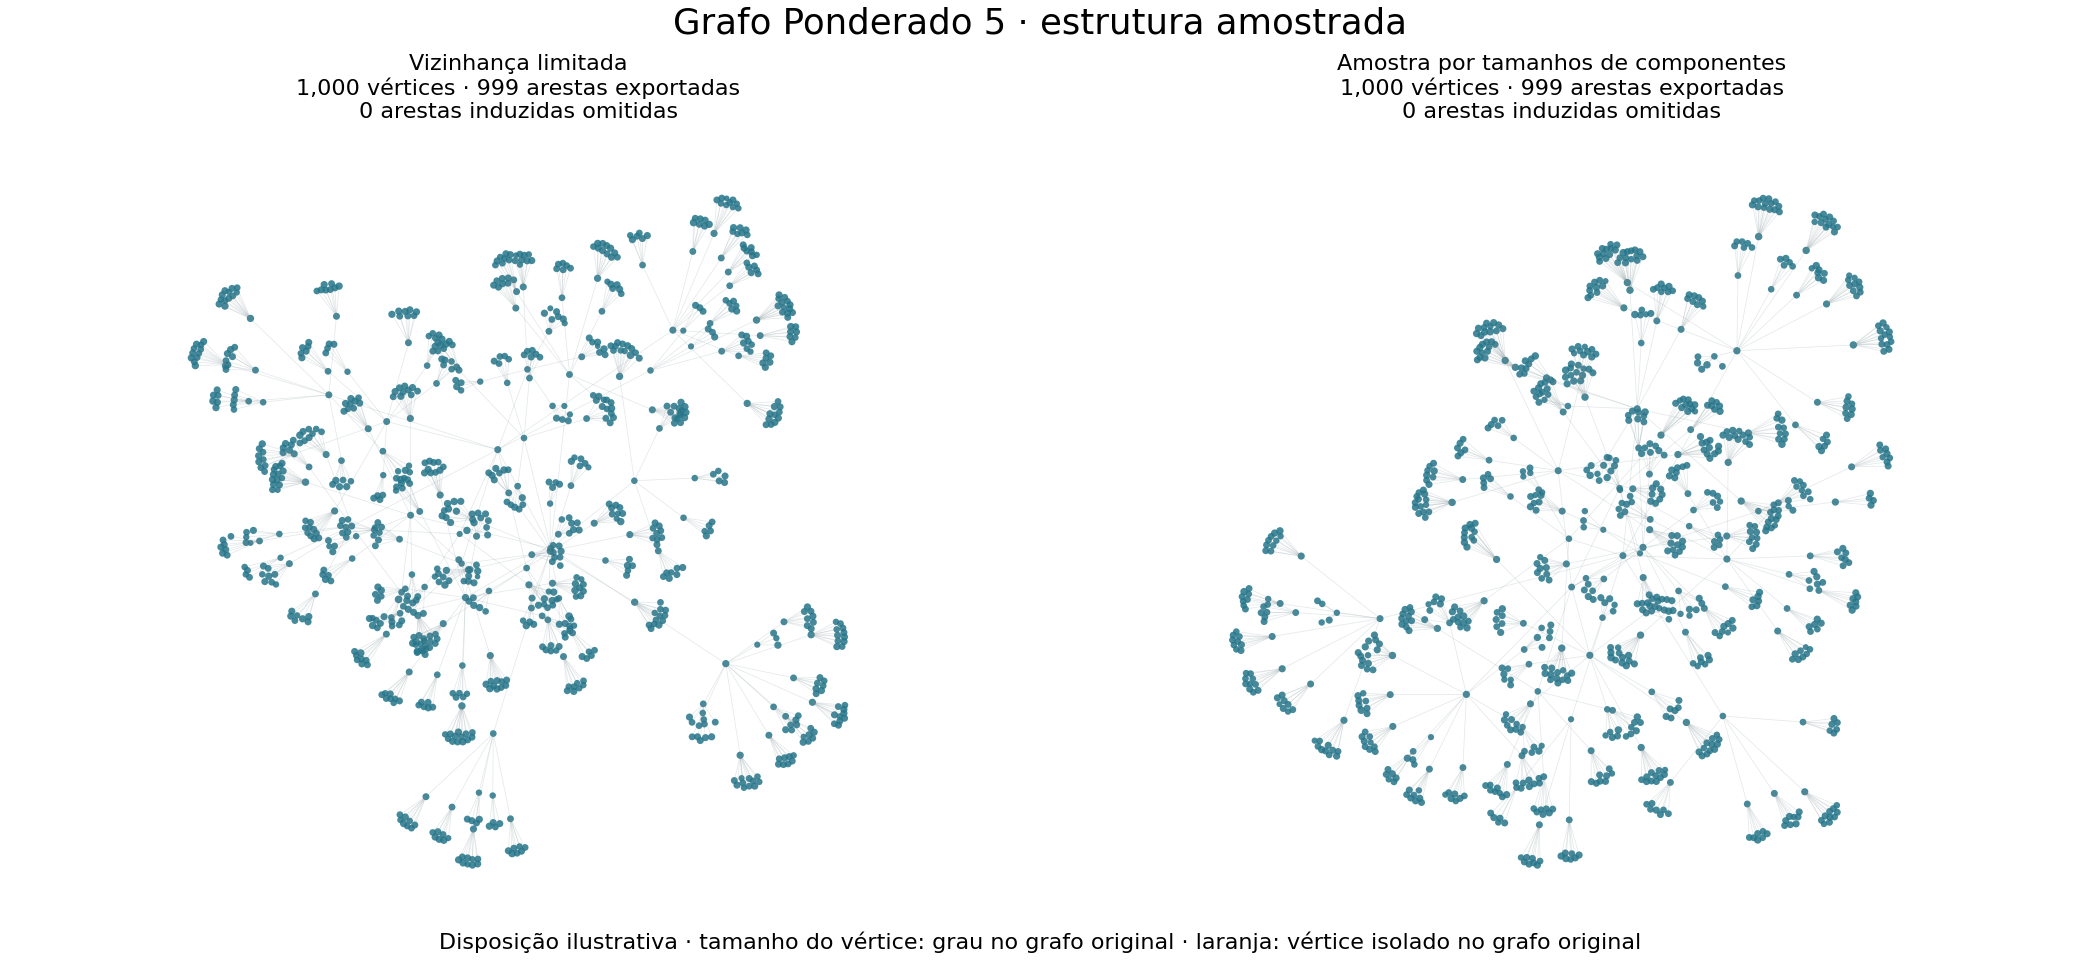
\includegraphics[width=\textwidth]{network_grafo_W_5.png}\caption{Estrutura amostrada de Grafo Ponderado 5. Os dois painéis não representam o grafo inteiro.}\end{figure}
\begin{figure}[H]\centering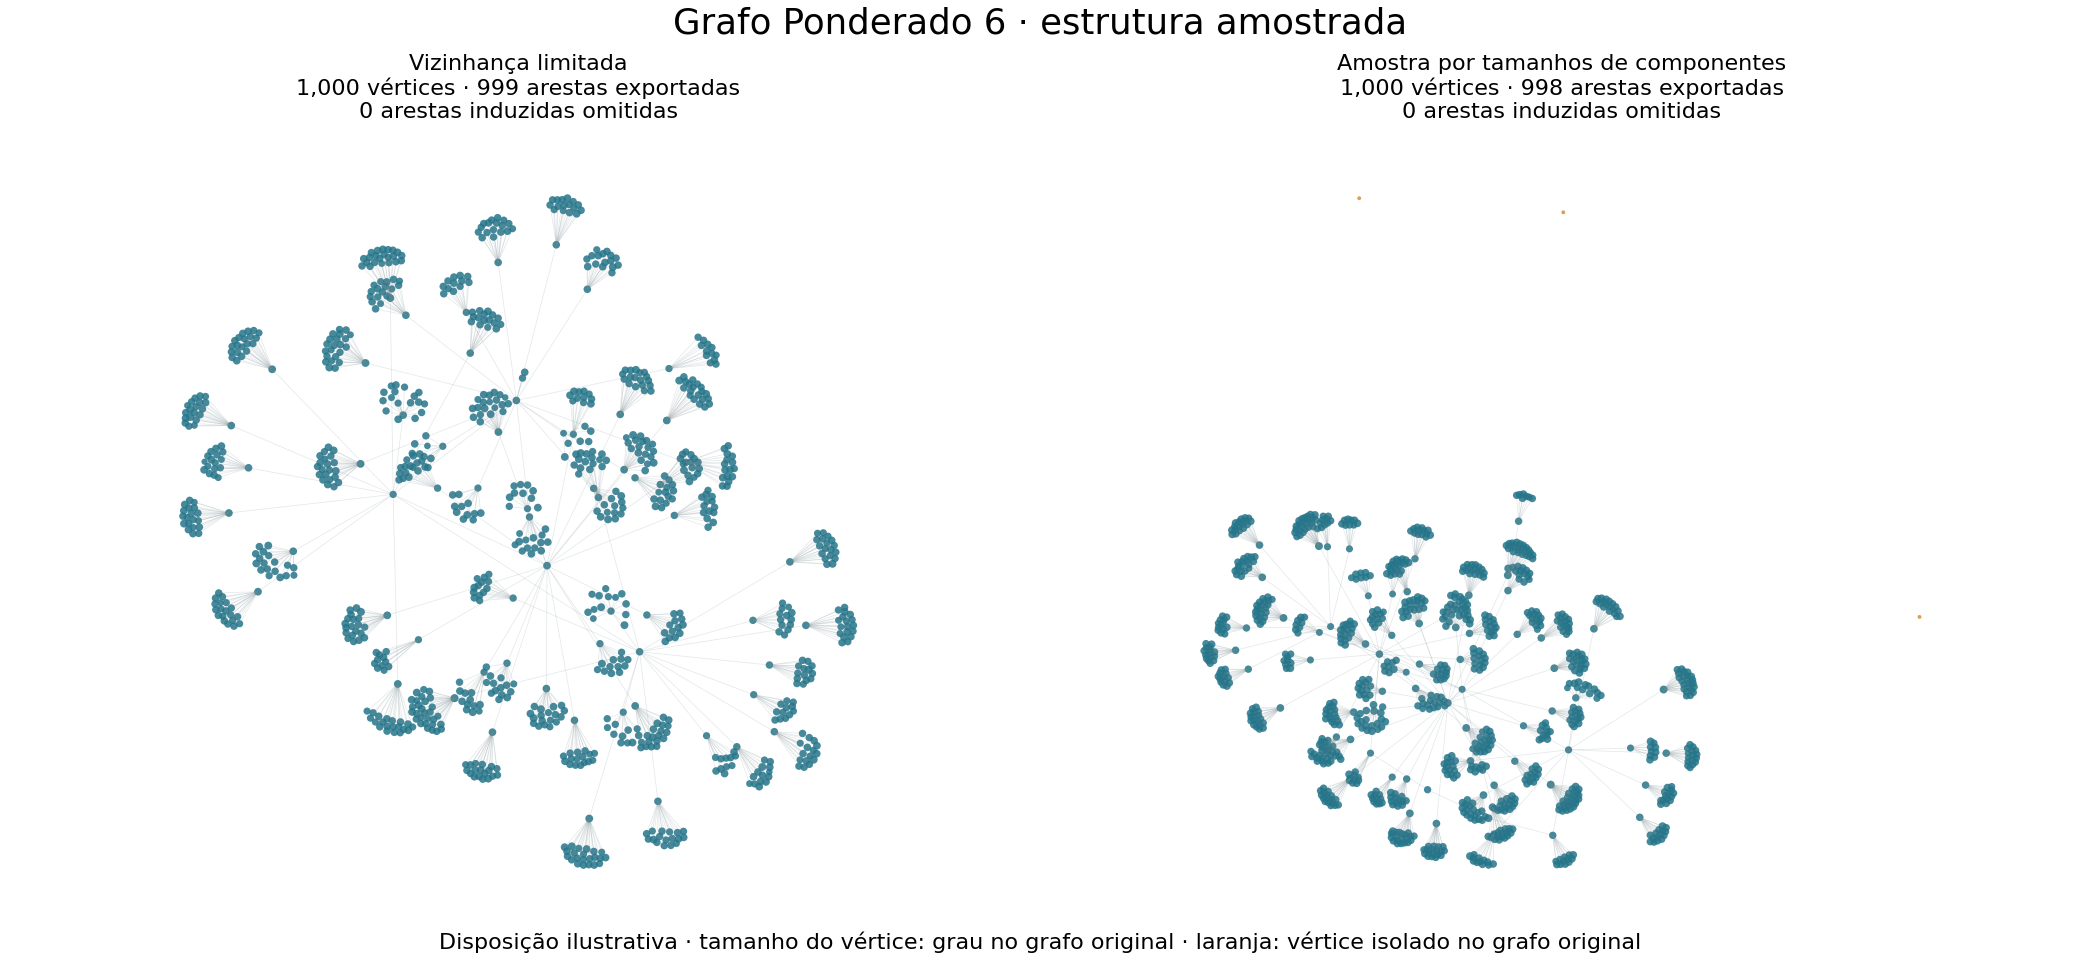
\includegraphics[width=\textwidth]{network_grafo_W_6.png}\caption{Estrutura amostrada de Grafo Ponderado 6. Os dois painéis não representam o grafo inteiro.}\end{figure}
\begin{figure}[H]\centering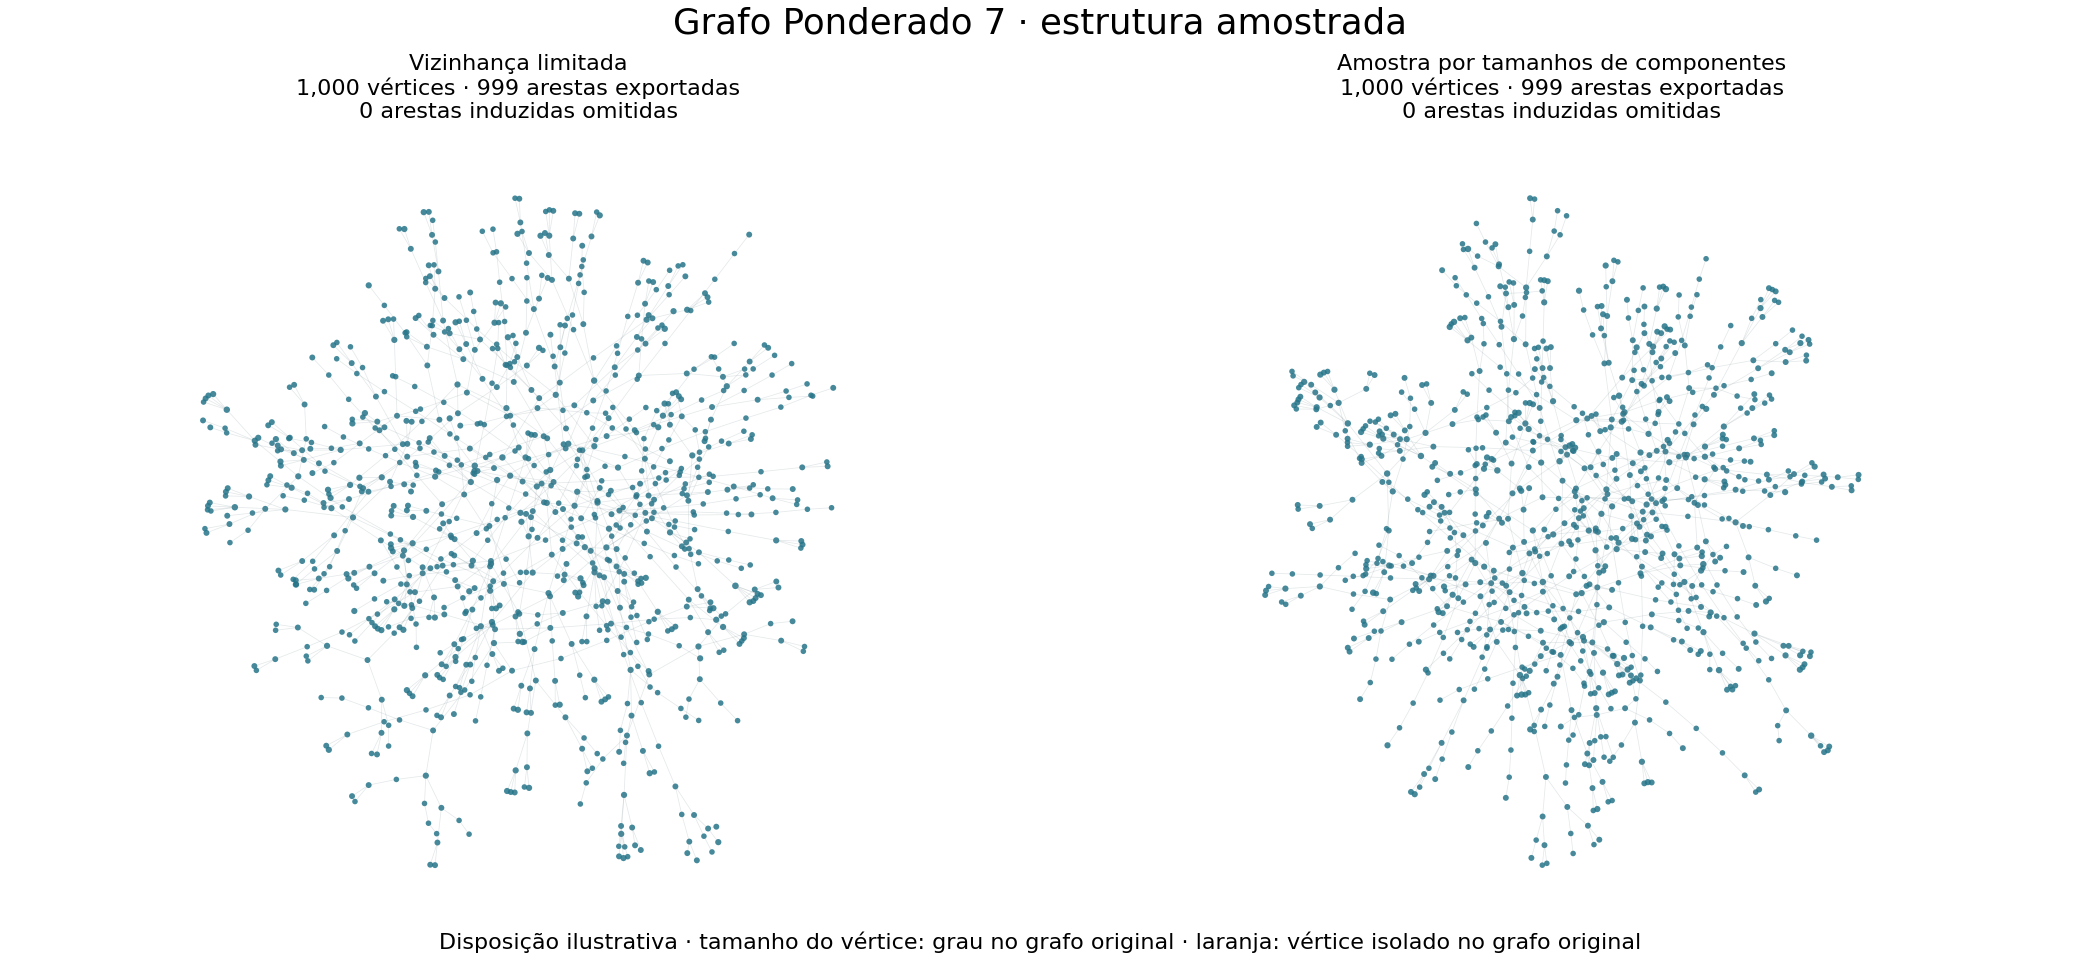
\includegraphics[width=\textwidth]{network_grafo_W_7.png}\caption{Estrutura amostrada de Grafo Ponderado 7. Os dois painéis não representam o grafo inteiro.}\end{figure}
\begin{figure}[H]\centering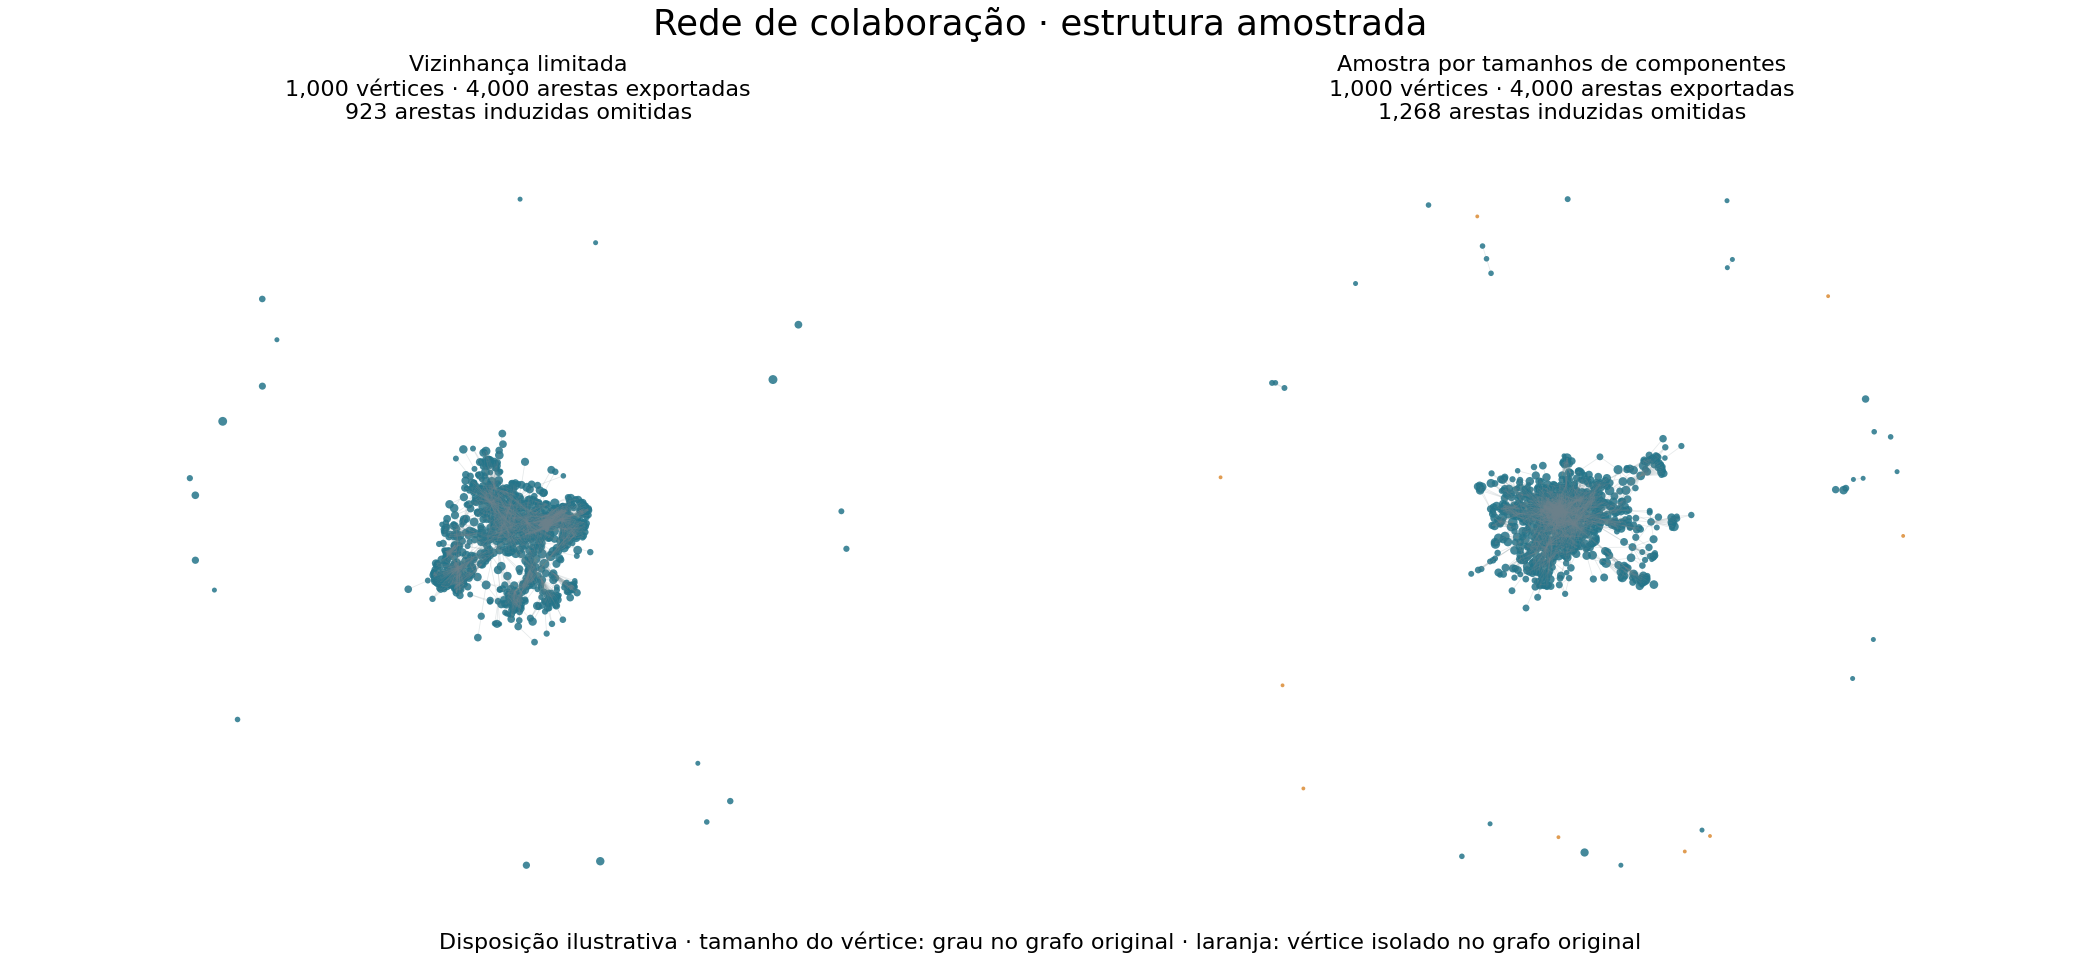
\includegraphics[width=\textwidth]{network_rede_colaboracao.png}\caption{Estrutura amostrada de Rede de colaboração. Os dois painéis não representam o grafo inteiro.}\end{figure}
\clearpage
\section{Casos artificiais de referência}
Os valores esperados foram calculados manualmente e registrados em \path{tests/data/baselines/manifest.json}. São casos de correção, não estimativas de desempenho para milhões de vértices. A origem é 1; vizinhos são visitados em ordem crescente. Os 11 casos geraram 160 resultados por vértice/algoritmo conferidos. O valor $-1$ indica inalcançabilidade nos níveis das buscas; $+\infty$ indica distância ponderada infinita. Para regenerar: \cod{make baselines}.
\par\noindent\begin{minipage}{\textwidth}\subsection{Vértice isolado}
Origem igual ao destino; profundidade zero e nenhuma aresta.
\par\smallskip\noindent\begin{minipage}{\textwidth}\centering
\begingroup\small
\setlength{\tabcolsep}{4pt}
\begin{tabular}{l>{\raggedright\arraybackslash}p{10.4cm}}
\toprule
Algoritmo & Valores por vértice, a partir de 1 \\
\midrule
BFS: distâncias & \num{0} \\
DFS: profundidades & \num{0} \\
\bottomrule
\end{tabular}
\endgroup
\end{minipage}\par\smallskip
\end{minipage}\par\medskip
\par\noindent\begin{minipage}{\textwidth}\subsection{Caminho linear}
BFS e DFS coincidem; diâmetro de cinco arestas.
\par\smallskip\noindent\begin{minipage}{\textwidth}\centering
\begingroup\small
\setlength{\tabcolsep}{4pt}
\begin{tabular}{l>{\raggedright\arraybackslash}p{10.4cm}}
\toprule
Algoritmo & Valores por vértice, a partir de 1 \\
\midrule
BFS: distâncias & \num{0}, \num{1}, \num{2}, \num{3}, \num{4}, \num{5} \\
DFS: profundidades & \num{0}, \num{1}, \num{2}, \num{3}, \num{4}, \num{5} \\
\bottomrule
\end{tabular}
\endgroup
\end{minipage}\par\smallskip
\end{minipage}\par\medskip
\par\noindent\begin{minipage}{\textwidth}\subsection{Estrela}
Alto grau central; todas as folhas têm distância um.
\par\smallskip\noindent\begin{minipage}{\textwidth}\centering
\begingroup\small
\setlength{\tabcolsep}{4pt}
\begin{tabular}{l>{\raggedright\arraybackslash}p{10.4cm}}
\toprule
Algoritmo & Valores por vértice, a partir de 1 \\
\midrule
BFS: distâncias & \num{0}, \num{1}, \num{1}, \num{1}, \num{1}, \num{1} \\
DFS: profundidades & \num{0}, \num{1}, \num{1}, \num{1}, \num{1}, \num{1} \\
\bottomrule
\end{tabular}
\endgroup
\end{minipage}\par\smallskip
\end{minipage}\par\medskip
\par\noindent\begin{minipage}{\textwidth}\subsection{Grafo completo}
BFS mantém distância um; DFS produz uma árvore profunda, com vizinhos em ordem crescente.
\par\smallskip\noindent\begin{minipage}{\textwidth}\centering
\begingroup\small
\setlength{\tabcolsep}{4pt}
\begin{tabular}{l>{\raggedright\arraybackslash}p{10.4cm}}
\toprule
Algoritmo & Valores por vértice, a partir de 1 \\
\midrule
BFS: distâncias & \num{0}, \num{1}, \num{1}, \num{1}, \num{1} \\
DFS: profundidades & \num{0}, \num{1}, \num{2}, \num{3}, \num{4} \\
\bottomrule
\end{tabular}
\endgroup
\end{minipage}\par\smallskip
\end{minipage}\par\medskip
\par\noindent\begin{minipage}{\textwidth}\subsection{Empate de caminhos e componente isolada}
Duas rotas mínimas; o vértice 5 é inalcançável. Distância correta independe do desempate entre pais.
\par\smallskip\noindent\begin{minipage}{\textwidth}\centering
\begingroup\small
\setlength{\tabcolsep}{4pt}
\begin{tabular}{l>{\raggedright\arraybackslash}p{10.4cm}}
\toprule
Algoritmo & Valores por vértice, a partir de 1 \\
\midrule
BFS: distâncias & \num{0}, \num{1}, \num{1}, \num{2}, \num{-1} \\
DFS: profundidades & \num{0}, \num{1}, \num{3}, \num{2}, \num{-1} \\
\bottomrule
\end{tabular}
\endgroup
\end{minipage}\par\smallskip
\end{minipage}\par\medskip
\par\noindent\begin{minipage}{\textwidth}\subsection{Menos arestas não significa menor peso}
BFS chega a 2 com uma aresta de peso 10; Dijkstra prefere duas arestas de peso total 2.
\par\smallskip\noindent\begin{minipage}{\textwidth}\centering
\begingroup\small
\setlength{\tabcolsep}{4pt}
\begin{tabular}{l>{\raggedright\arraybackslash}p{10.4cm}}
\toprule
Algoritmo & Valores por vértice, a partir de 1 \\
\midrule
BFS: distâncias & \num{0}, \num{1}, \num{1}, \num{-1} \\
DFS: profundidades & \num{0}, \num{1}, \num{2}, \num{-1} \\
Dijkstra: três versões & \num{0}, \num{2}, \num{1}, $+\infty$ \\
\bottomrule
\end{tabular}
\endgroup
\end{minipage}\par\smallskip
\end{minipage}\par\medskip
\par\noindent\begin{minipage}{\textwidth}\subsection{Ciclo de peso zero}
O ciclo de peso zero deve terminar sem formar ciclos nos pais; o vértice 5 permanece inalcançável.
\par\smallskip\noindent\begin{minipage}{\textwidth}\centering
\begingroup\small
\setlength{\tabcolsep}{4pt}
\begin{tabular}{l>{\raggedright\arraybackslash}p{10.4cm}}
\toprule
Algoritmo & Valores por vértice, a partir de 1 \\
\midrule
BFS: distâncias & \num{0}, \num{1}, \num{1}, \num{2}, \num{-1} \\
DFS: profundidades & \num{0}, \num{1}, \num{2}, \num{3}, \num{-1} \\
Dijkstra: três versões & \num{0}, \num{0}, \num{0}, \num{2}, $+\infty$ \\
\bottomrule
\end{tabular}
\endgroup
\end{minipage}\par\smallskip
\end{minipage}\par\medskip
\par\noindent\begin{minipage}{\textwidth}\subsection{Reduções sucessivas de chave}
A estimativa para 2 diminui de 20 para 11 e depois 3; exercita update\_key e entradas obsoletas da versão tardia.
\par\smallskip\noindent\begin{minipage}{\textwidth}\centering
\begingroup\small
\setlength{\tabcolsep}{4pt}
\begin{tabular}{l>{\raggedright\arraybackslash}p{10.4cm}}
\toprule
Algoritmo & Valores por vértice, a partir de 1 \\
\midrule
BFS: distâncias & \num{0}, \num{1}, \num{1}, \num{1}, \num{-1} \\
DFS: profundidades & \num{0}, \num{1}, \num{2}, \num{3}, \num{-1} \\
Dijkstra: três versões & \num{0}, \num{3}, \num{2}, \num{1}, $+\infty$ \\
\bottomrule
\end{tabular}
\endgroup
\end{minipage}\par\smallskip
\end{minipage}\par\medskip
\par\noindent\begin{minipage}{\textwidth}\subsection{Caminhos ponderados empatados}
Empates de distância não exigem árvores de pais idênticas nas três versões.
\par\smallskip\noindent\begin{minipage}{\textwidth}\centering
\begingroup\small
\setlength{\tabcolsep}{4pt}
\begin{tabular}{l>{\raggedright\arraybackslash}p{10.4cm}}
\toprule
Algoritmo & Valores por vértice, a partir de 1 \\
\midrule
BFS: distâncias & \num{0}, \num{1}, \num{1}, \num{2} \\
DFS: profundidades & \num{0}, \num{1}, \num{3}, \num{2} \\
Dijkstra: três versões & \num{0}, \num{1}, \num{1}, \num{2} \\
\bottomrule
\end{tabular}
\endgroup
\end{minipage}\par\smallskip
\end{minipage}\par\medskip
\par\noindent\begin{minipage}{\textwidth}\subsection{Arestas paralelas e laço}
O leitor descarta o laço; CSR preserva as paralelas e Dijkstra encontra a de menor peso.
\par\smallskip\noindent\begin{minipage}{\textwidth}\centering
\begingroup\small
\setlength{\tabcolsep}{4pt}
\begin{tabular}{l>{\raggedright\arraybackslash}p{10.4cm}}
\toprule
Algoritmo & Valores por vértice, a partir de 1 \\
\midrule
BFS: distâncias & \num{0}, \num{1}, \num{2} \\
DFS: profundidades & \num{0}, \num{1}, \num{2} \\
Dijkstra: três versões & \num{0}, \num{2}, \num{3} \\
\bottomrule
\end{tabular}
\endgroup
\end{minipage}\par\smallskip
\end{minipage}\par\medskip
\par\noindent\begin{minipage}{\textwidth}\subsection{Aresta negativa}
BFS e DFS ignoram pesos; as três versões de Dijkstra devem rejeitar a entrada.
\par\smallskip\noindent\begin{minipage}{\textwidth}\centering
\begingroup\small
\setlength{\tabcolsep}{4pt}
\begin{tabular}{l>{\raggedright\arraybackslash}p{10.4cm}}
\toprule
Algoritmo & Valores por vértice, a partir de 1 \\
\midrule
BFS: distâncias & \num{0}, \num{1}, \num{2} \\
DFS: profundidades & \num{0}, \num{1}, \num{2} \\
Dijkstra: três versões & Rejeição esperada por peso negativo \\
\bottomrule
\end{tabular}
\endgroup
\end{minipage}\par\smallskip
\end{minipage}\par\medskip
\section{Rastreabilidade e reprodução}
O gerador \path{analysis/build_report_part2.py} lê apenas resultados salvos, verifica os 30 pares e os resumos e produz os dois fontes LaTeX. Não executa Dijkstra, BFS, DFS nem provisiona recursos. Os arquivos \path{data/azure/results_weighted.csv} e \cod{paths_weighted.csv} são da rodada histórica. Os resumos da nova rodada estão em \path{docs/results/traversals/}, e os brutos, fontes e executável Linux, em \path{data/azure_traversals/}. Este último diretório e os grandes dados de entrada não são versionados.

\path{docs/figures/provenance.json} contém hashes das figuras, dados e scripts de visualização. \path{docs/results/traversals/execution_record.json} registra execução e limpeza. As estatísticas estruturais foram calculadas separadamente das medições de tempo no Azure; não são medições de desempenho local apresentadas como nuvem. O ambiente do relatório deve ser analisado por rodada, pois código, caches e alocador podem mudar mesmo numa VM da mesma categoria.

Os fontes LaTeX usam PNGs da galeria no complemento; o relatório principal é independente de imagens externas. A compilação com Tectonic pode ser feita a partir da raiz do repositório. O diagrama Mermaid detalha a arquitetura atual; o diagrama anterior foi preservado em seu arquivo original. A biblioteca não foi alterada para produzir este material.
\end{document}
